% 无线电/无线电基础知识
% 0_无线电基础知识.tex

\documentclass[12pt,UTF8]{ctexbook}

% 设置纸张信息。
\input{../../../../common/page}

% 设置字体，并解决显示难检字问题。
\xeCJKsetup{AutoFallBack=true}
\setCJKmainfont{SimSun}[BoldFont=SimHei, ItalicFont=KaiTi, FallBack=SimSun-ExtB]

% 数学符号支持
\usepackage{amsfonts}
\usepackage{amssymb}

% 表格支持
\usepackage{threeparttable}

% 目录 chapter 级别加点（.）。
\usepackage{titletoc}
\titlecontents{chapter}[0pt]{\vspace{3mm}\bf\addvspace{2pt}\filright}{\contentspush{\thecontentslabel\hspace{0.8em}}}{}{\titlerule*[8pt]{.}\contentspage}

% 支持目录点击跳转
\usepackage[colorlinks,linkcolor=blue,citecolor=blue,urlcolor=blue]{hyperref}

% 设置 part 和 chapter 标题格式。
\ctexset{
	part/name={第,部分},
	part/number={\arabic{part}},
	chapter/name={第,章},
	chapter/number={\arabic{chapter}}
}

% 列表格式支持
\usepackage{enumitem}

% 数学公式支持
\usepackage{amsmath}

% 图片相关设置。
\usepackage{graphicx}
\graphicspath{{Images/}}

% 设置署名格式。
\newenvironment{shuming}{\hfill\zihao{4}}

% 注脚每页重新编号，避免编号过大。
\usepackage[perpage]{footmisc}

% 索引功能
\usepackage{makeidx}
\makeindex

% 段落间距设置
\usepackage{setspace}
\onehalfspacing % 设置1.5倍行间距
\setlength{\parskip}{1em} % 设置段落间距

\title{\heiti\zihao{0} 无线电基础}
\author{王飞}
\date{}

\begin{document}

\maketitle
\tableofcontents
\listoffigures
\listoftables

\frontmatter

\mainmatter

\part{无线电基础理论}

\chapter{无线电基础概述}

本章介绍无线电技术的基本概念和发展历程，为后续章节的学习奠定基础。主要内容包括无线电的基本概念、技术原理和理论体系，帮助读者建立对无线电技术的整体认识。

\section{无线电的基本概念}

无线电技术是利用电磁波在空间中传播信息的技术，是现代通信技术的基础。无线电技术基于电磁波理论，通过调制解调技术实现信息的无线传输。

无线电技术的发展经历了从电磁波理论的建立到现代通信技术的漫长历程：
\begin{itemize}[leftmargin=3.5em]
    \item 19世纪60年代，麦克斯韦建立了电磁场理论，预言了电磁波的存在
    \item 1887年，赫兹通过实验验证了电磁波的存在
    \item 1895年，马可尼成功实现了无线电报通信
    \item 20世纪初，无线电广播开始普及
    \item 20世纪中期，电视和雷达技术得到发展
    \item 20世纪后期，数字通信技术迅速发展
    \item 21世纪初，3G/4G移动通信技术大规模应用
    \item 2010年代，5G通信技术研发和商用部署
    \item 2020年代，6G、太赫兹通信、空天地一体化网络等前沿技术研究加速
\end{itemize}

\section{无线电技术的基本原理}

无线电技术基于以下基本原理：

\begin{itemize}[leftmargin=3.5em]
    \item \textbf{电磁波理论}：麦克斯韦方程组描述的电磁场理论，是无线电技术的理论基础
    \item \textbf{调制解调}：将信息信号调制到载波上的技术，实现信息的有效传输
    \item \textbf{频谱分析}：电磁波在频域的分布特性，用于信号的分析和处理
    \item \textbf{传播特性}：电磁波在不同介质中的传播规律，影响信号的传输质量
\end{itemize}

\chapter{电磁波基础}

本章介绍电磁波的基本理论和特性，包括电磁波的产生、传播规律和数学描述。电磁波是无线电技术的基础，理解电磁波特性对于掌握无线电技术至关重要。主要内容包括电磁波的基本特性、数学描述、参数计算和频谱分析。

\section{电磁波的基本特性}

电磁波是由变化的电场和磁场相互激发而形成的波动现象。1864年，英国物理学家麦克斯韦建立了电磁场理论，预言了电磁波的存在。1887年，德国物理学家赫兹通过实验证实了电磁波的存在。电磁波在空间中以光速传播，不需要介质，可以在真空中传播。

麦克斯韦于1873年提出了统一的电磁场理论，即振荡电路发生电磁振荡时，就向空间发射电磁波，而这些波在空间以光速向外传播。

赫兹从实验上证实了这理论的正确性。他提出：任何变化的电场都会在它周围的空间产生磁场；同样，任何变化的磁场也会在它周围的空间产生电场。

根据这论点，假设某空间或某区域发生周期性变化的电场，就在它邻近区域引起周期性变化的磁场，这个周期性变化的磁场又要在它较远的区域中引起新的周期性变化的电场，电场和磁场就是这样交替变化着向远方传播出去。

\begin{figure}[htbp]
    \centering
    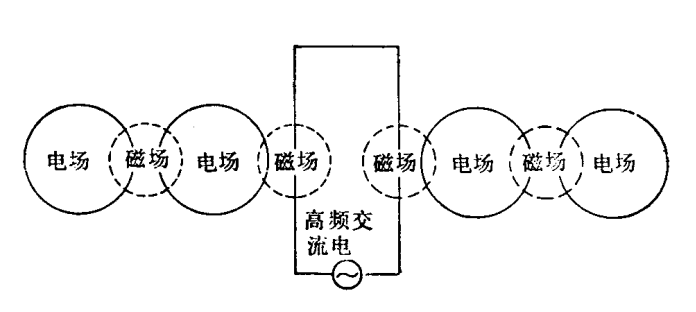
\includegraphics[width=0.7\linewidth]{electromagnetic_wave.png}
    \caption{电磁波传播示意图}
    \label{fig:electromagnetic_wave}
\end{figure}

电磁波的基本特性包括频率、波长、振幅、相位和偏振等。频率是指电磁波每秒振荡的次数，单位是赫兹（Hz）。波长是指电磁波一个完整周期在空间中传播的距离，单位是米（m）。频率和波长成反比关系，即频率越高，波长越短。振幅是指电磁波的最大强度，决定了信号的强弱。相位是指电磁波在某个时刻的状态，用于描述波的相对位置。偏振是指电磁波电场矢量的振动方向。

电磁波的频谱非常宽广，从极低频的无线电波到极高频的伽马射线，频率范围从几赫兹到$10^{24}$赫兹。无线电波是电磁波频谱中频率较低的部分，频率范围从$3\,\text{kHz}$到$300\,\text{GHz}$。根据频率和波长的不同，无线电波被划分为多个频段，每个频段具有不同的传播特性和应用领域。

电磁波具有以下基本特性：

\begin{itemize}[leftmargin=3.5em]
    \item \textbf{波动性}：具有波长、频率、振幅等波动特性
    \item \textbf{传播性}：可以在真空中以光速传播
    \item \textbf{反射性}：遇到障碍物会发生反射
    \item \textbf{折射性}：在不同介质中传播会发生折射
    \item \textbf{衍射性}：遇到障碍物边缘会发生衍射
    \item \textbf{干涉性}：多列波叠加会产生干涉现象
\end{itemize}

电磁波的传播遵循麦克斯韦方程组，描述了电场和磁场的变化规律。电磁波在传播过程中会发生反射、折射、衍射、干涉等现象，这些现象对无线电接收设备的接收效果有重要影响。了解电磁波的基本原理，对于理解无线电系统的工作原理和优化接收效果非常重要。

\section{电磁波的数学描述}

电磁波可以用麦克斯韦方程组进行精确描述，这是电磁理论的基础：

\begin{itemize}[leftmargin=3.5em]
    \item \textbf{高斯定律}：描述电场的散度与电荷密度的关系
    \item \textbf{高斯磁定律}：表明磁场是无源场，不存在磁单极子
    \item \textbf{法拉第定律}：描述变化的磁场产生电场
    \item \textbf{安培-麦克斯韦定律}：描述电流和变化的电场产生磁场
\end{itemize}

麦克斯韦方程组的数学表达式为：
\begin{align}
\nabla \cdot \mathbf{E} &= \frac{\rho}{\varepsilon_0} \\
\nabla \cdot \mathbf{B} &= 0 \\
\nabla \times \mathbf{E} &= -\frac{\partial \mathbf{B}}{\partial t} \\
\nabla \times \mathbf{B} &= \mu_0\mathbf{J} + \mu_0\varepsilon_0\frac{\partial \mathbf{E}}{\partial t} \\ 
\end{align}

从麦克斯韦方程组可以推导出电磁波的波动方程：
\begin{align}
\nabla^2 \mathbf{E} &= \mu_0\varepsilon_0 \frac{\partial^2 \mathbf{E}}{\partial t^2} \\
\nabla^2 \mathbf{B} &= \mu_0\varepsilon_0 \frac{\partial^2 \mathbf{B}}{\partial t^2} \\ 
\end{align}

其中波速 $v = \frac{1}{\sqrt{\mu_0\varepsilon_0}} = c$，即光速。

\section{电磁波参数计算}

电磁波的关键参数可以通过以下公式计算：

\begin{itemize}[leftmargin=3.5em]
    \item \textbf{波长计算}：$\lambda = \frac{c}{f}$，其中$c=3\times10^8$ m/s为光速，$f$为频率
    \item \textbf{周期计算}：$T = \frac{1}{f}$，表示波完成一个完整振荡所需的时间
    \item \textbf{波数计算}：$k = \frac{2\pi}{\lambda}$，表示单位长度内的波周期数
    \item \textbf{角频率计算}：$\omega = 2\pi f$，表示单位时间内的角度变化
    \item \textbf{波阻抗计算}：$Z = \sqrt{\frac{\mu}{\varepsilon}}$，在真空中约为377Ω
\end{itemize}

例如，对于频率为$100\,\text{MHz}$的电磁波：
\begin{itemize}[leftmargin=3.5em]
    \item 波长：$\lambda = \frac{3\times10^8}{100\times10^6} = 3$米
    \item 周期：$T = \frac{1}{100\times10^6} = 10$纳秒
    \item 波数：$k = \frac{2\pi}{3} \approx 2.09$ rad/m
    \item 角频率：$\omega = 2\pi \times 100\times10^6 \approx 6.28\times10^8$ rad/s
\end{itemize}

另一个示例，对于5G通信中常用的$3.5\,\text{GHz}$频段：
\begin{itemize}[leftmargin=3.5em]
    \item 频率：$f = 3.5$ GHz = $3.5\times10^9$ Hz
    \item 波长：$\lambda = \frac{3\times10^8}{3.5\times10^9} \approx 0.0857$米 = 8.57厘米
    \item 周期：$T = \frac{1}{3.5\times10^9} \approx 0.286$纳秒
    \item 波数：$k = \frac{2\pi}{0.0857} \approx 73.5$ rad/m
    \item 角频率：$\omega = 2\pi \times 3.5\times10^9 \approx 2.2\times10^{10}$ rad/s
\end{itemize}

\section{电磁波频谱}

电磁波频谱按照频率从低到高可以分为：

\begin{itemize}[leftmargin=3.5em]
    \item \textbf{无线电波}：$3\,\text{kHz}$-$300\,\text{GHz}$，用于通信、广播、导航和遥感
    \item \textbf{微波}：$300\,\text{MHz}$-$300\,\text{GHz}$，用于雷达、卫星通信、微波炉和无线局域网
    \item \textbf{红外线}：$300\,\text{GHz}$-$430\,\text{THz}$，用于热成像、遥控、安防和医疗
    \item \textbf{可见光}：$430\,\text{THz}$-$750\,\text{THz}$，人眼可见的光波，用于照明和显示
    \item \textbf{紫外线}：$750\,\text{THz}$-$30\,\text{PHz}$，用于杀菌、荧光检测和医疗消毒
    \item \textbf{X射线}：$30\,\text{PHz}$-$30\,\text{EHz}$，用于医疗诊断、材料检测和安全检查
    \item \textbf{伽马射线}：$30\,\text{EHz}$以上，用于核物理研究、医疗治疗和工业探伤
\end{itemize}

现代无线电技术的重要应用频段：
\begin{itemize}[leftmargin=3.5em]
    \item \textbf{5G通信}：3.5GHz、2.6GHz频段，大规模MIMO技术，超高速率低时延
    \item \textbf{毫米波通信}：24-100GHz频段，支持太比特级传输速率
    \item \textbf{Wi-Fi 6/7}：2.4GHz、5GHz、6GHz频段，更高的吞吐量和更低的延迟
    \item \textbf{卫星互联网}：Ku/Ka频段，实现全球无缝覆盖
    \item \textbf{物联网}：Sub-GHz、2.4GHz频段，低功耗广域覆盖
\end{itemize}

\subsection{无线电波的频段划分}

无线电波的频段划分有传统分类和现代标准分类两种方式。以下是综合的频段划分表：

\begin{table}[htbp]
    \centering
    \begin{threeparttable}
    \small
    \begin{tabular}{|p{2cm}|p{1.2cm}|p{3cm}|p{2cm}|p{4cm}|}
        \hline
        \textbf{频段名称} & \textbf{英文缩写} & \textbf{频率范围} & \textbf{波长范围} & \textbf{主要用途} \\
        \hline
        极低频/超长波 & VLF & 3-30kHz & 10-100km & 水下通信、无线电导航 \\
        \hline
        低频/长波 & LF & 30-300kHz & 1-10km & 长波广播、无线电导航 \\
        \hline
        中频/中波 & MF & 300kHz-3MHz & 100-1000m & 中波广播（AM广播） \\
        \hline
        高频/短波 & HF & 3-30MHz & 10-100m & 短波广播、业余无线电、国际通讯 \\
        \hline
        甚高频/超短波 & VHF & 30-300MHz & 1-10m & 调频广播（FM广播）、电视广播、航空通信 \\
        \hline
        特高频 & UHF & 300MHz-3GHz & 0.1-1m & 移动通信、电视广播、卫星通信 \\
        \hline
        超高频 & SHF & 3-30GHz & 1-10cm & 卫星通信、雷达、微波通信、5G通信 \\
        \hline
        极高频 & EHF & 30-300GHz & 1-10mm & 卫星通信、科学研究、毫米波通信 \\
        \hline
    \end{tabular}
    \caption{综合无线电频段划分表}
    \label{tab:radio_bands_comprehensive}
    \begin{tablenotes}
        \item[注1] 中短波（1500-6000kHz）属于MF和HF频段的重叠区域，主要用于电报通讯和广播。
        \item[注2] 微波通常指波长小于1米（频率高于300MHz）的电磁波，包括UHF、SHF和EHF频段，具有频带宽、信息容量大、直线传播等特点。
    \end{tablenotes}
    \end{threeparttable}
\end{table}

\section{练习与思考}

1. 什么是电磁波？它是如何产生和传播的？
2. 电磁波的频率和波长之间有什么关系？请推导它们的关系式。
3. 计算频率为2.4GHz的电磁波的波长。
4. 电磁波在真空中的传播速度是多少？在其他介质中呢？
5. 电磁波的基本特性有哪些？
6. 无线电波的频率范围是多少？如何分类？
7. 微波的特点是什么？在通信中有哪些应用？
8. 电磁波的偏振是什么意思？有哪些类型？
9. 电磁波的能量是如何传播的？
10. 麦克斯韦方程组的物理意义是什么？



\chapter{天线基础}

本章介绍天线的基本原理、类型和设计方法。天线是无线电系统的关键组件，负责电磁波的发射和接收。主要内容包括天线的基本原理、常见天线类型、天线参数计算和天线阵列技术。

\section{天线的基本原理}

天线是无线电系统中用于发射和接收电磁波的设备，其工作原理基于电磁感应定律：当变化的电磁场通过导体时，会在导体中感应出电流。天线的基本功能是实现电磁波与电信号之间的转换。

天线的主要参数包括：

\begin{itemize}[leftmargin=3.5em]
    \item \textbf{增益}：天线在特定方向上的辐射或接收能力，相对于参考天线（如偶极子天线）的增益
    \item \textbf{方向性}：天线在不同方向上的辐射或接收能力不同，有些天线是全向的，有些是定向的
    \item \textbf{阻抗}：天线的输入阻抗，需要与传输线和接收电路的阻抗匹配，以获得最大功率传输
    \item \textbf{带宽}：天线能够有效工作的频率范围
    \item \textbf{驻波比}：衡量天线阻抗匹配程度的指标，驻波比越接近1，匹配越好
\end{itemize}

天线的长度与工作信号的波长有关。对于半波偶极子天线，其长度约为工作信号波长的一半。对于四分之一波长垂直天线，其长度约为工作信号波长的四分之一。天线越长，接收低频信号的效果越好；天线越短，接收高频信号的效果越好。

了解天线的基本原理和参数，对于选择合适的无线通信天线、优化通信效果非常重要。不同的通信环境和通信需求，需要使用不同类型和规格的天线。

\section{常见天线类型}

天线类型多种多样，根据不同的分类标准可以分为不同的类型：

\textbf{按结构分类}：
\begin{itemize}[leftmargin=3.5em]
    \item \textbf{偶极子天线}：最基本的天线类型，由两根长度相等、方向相反的导体组成，长度约为工作信号波长的一半，具有简单的结构、良好的性能和适中的增益
    \item \textbf{单极子天线}：偶极子天线的一半，由一根垂直导体组成，长度约为工作信号波长的四分之一，常用于移动设备和便携设备
    \item \textbf{环形天线}：由一个或多个环形导体组成，具有方向性好、抗干扰能力强等优点，常用于定向接收
    \item \textbf{八木天线}：由一个有源振子和多个无源振子组成，具有高增益和强方向性，用于远距离通信
    \item \textbf{对数周期天线}：宽带天线，能够在较宽的频率范围内工作，适用于多频段应用
    \item \textbf{微带天线}：平面结构，便于集成，用于移动设备
\end{itemize}

\textbf{按安装方式分类}：
\begin{itemize}[leftmargin=3.5em]
    \item \textbf{室内天线}：主要用于室内接收，体积小，便于安装，但接收效果受室内环境影响较大
    \item \textbf{室外天线}：安装在室外，接收效果好，但安装复杂，需要考虑防雷、防水等问题
    \item \textbf{车载天线}：专为汽车设计，具有抗振动、抗干扰等特点
    \item \textbf{便携天线}：体积小，重量轻，便于携带，适合户外使用
\end{itemize}

\textbf{按工作频段分类}：
\begin{itemize}[leftmargin=3.5em]
    \item \textbf{长波天线}：适用于长波频段通信
    \item \textbf{中波天线}：适用于中波广播频段
    \item \textbf{短波天线}：适用于短波通信和广播
    \item \textbf{超短波天线}：适用于超短波通信和广播
\end{itemize}

选择合适的天线类型，需要考虑以下因素：

\begin{itemize}[leftmargin=3.5em]
    \item \textbf{工作频段}：不同频段需要不同类型的天线，如长波需要大型天线，而微波可以使用小型天线
    \item \textbf{通信环境}：室内环境适合使用小型天线，室外环境可以使用大型定向天线
    \item \textbf{通信距离}：短距离通信可以使用低增益天线，长距离通信需要高增益定向天线
    \item \textbf{安装条件}：空间受限的场合需要小型天线，空间充足的场合可以使用大型天线
    \item \textbf{成本预算}：不同类型天线的成本差异较大，需要根据预算选择合适的天线
\end{itemize}

\subsection{天线选择的实际案例}

\begin{itemize}[leftmargin=3.5em]
    \item \textbf{家用电视接收}：通常使用八木天线或对数周期天线，安装在屋顶或阳台
    \item \textbf{移动通信基站}：使用定向天线阵列，实现信号的定向覆盖
    \item \textbf{卫星通信}：使用抛物面天线，实现与卫星的通信
    \item \textbf{业余无线电}：根据频段不同选择偶极子、八木或环形天线
    \item \textbf{车载通信}：使用车载鞭状天线或吸盘天线，方便安装和移动
\end{itemize}

\section{天线设计与参数计算}

天线设计是无线电系统设计的重要组成部分，直接影响通信性能。天线设计需要考虑工作频率、增益、方向性、阻抗匹配、带宽、尺寸、成本等多种因素。好的天线设计能够在满足性能要求的前提下，实现体积小、成本低、易于安装的目标。

\textbf{天线设计基本步骤}：
\begin{itemize}[leftmargin=3.5em]
    \item \textbf{确定设计要求}：明确工作频率、增益要求、方向性要求、安装条件等
    \item \textbf{选择天线类型}：根据设计要求选择合适的偶极子、环形、八木等天线类型
    \item \textbf{计算天线尺寸}：根据工作频率计算天线尺寸，如偶极子天线长度约为波长的一半
    \item \textbf{优化天线参数}：通过仿真软件或实验方法优化增益、方向性、阻抗匹配等参数
    \item \textbf{制作原型测试}：制作天线原型，测量性能参数，根据测试结果调整设计
\end{itemize}

\textbf{天线关键参数计算}：
\begin{itemize}[leftmargin=3.5em]
    \item \textbf{偶极子天线长度}：$L = \frac{\lambda}{2}$，其中$\lambda$为工作波长
    \item \textbf{单极子天线长度}：$L = \frac{\lambda}{4}$，需要接地平面配合使用
    \item \textbf{天线效率}：$\eta = \frac{P_{rad}}{P_{in}}$，表示输入功率转换为辐射功率的比例
    \item \textbf{方向性系数}：$D = \frac{4\pi}{\Omega_A}$，其中$\Omega_A$为天线波束立体角
    \item \textbf{增益计算}：$G = \eta \cdot D$，综合考虑效率和方向性
    \item \textbf{有效面积}：$A_e = \frac{\lambda^2}{4\pi}G$，表示天线接收电磁波的有效面积
\end{itemize}

例如，对于工作频率为100MHz的偶极子天线：
\begin{itemize}[leftmargin=3.5em]
    \item 波长：$\lambda = \frac{3\times10^8}{100\times10^6} = 3$米
    \item 天线长度：$L = \frac{3}{2} = 1.5$米
    \item 如果天线效率为80\%，方向性系数为2.15dBi，则增益为：$G = 0.8 \times 10^{2.15/10} \approx 1.3$
\end{itemize}

另一个示例，对于5G通信中常用的3.5GHz频段：
\begin{itemize}[leftmargin=3.5em]
    \item 频率：$f = 3.5$ GHz
    \item 波长：$\lambda = \frac{3\times10^8}{3.5\times10^9} \approx 0.0857$米 = 8.57厘米
    \item 半波偶极子天线长度：$L = \frac{\lambda}{2} \approx 4.29$厘米
    \item 四分之一波长单极子天线长度：$L = \frac{\lambda}{4} \approx 2.14$厘米
    \item 有效面积：假设增益为5dBi，则$A_e = \frac{\lambda^2}{4\pi}G \approx \frac{(0.0857)^2}{4\pi} \times 3.16 \approx 0.00018$平方米
\end{itemize}

天线尺寸计算后，需要通过仿真软件或实验方法优化天线的参数，如增益、方向性、阻抗匹配、带宽等。常用的天线仿真软件有HFSS、CST、NEC等。优化完成后，制作天线原型，进行实际测试，测量天线的性能参数，如增益、方向图、驻波比等。根据测试结果调整天线设计，直到满足设计要求。

天线设计中需要注意的问题包括阻抗匹配、带宽优化、尺寸控制、成本控制等。

\textbf{天线匹配技术}：

天线匹配是指将天线的输入阻抗与传输线和接收电路的阻抗匹配，以获得最大功率传输和最小的信号反射。阻抗匹配是天线系统设计中的重要环节，直接影响通信效果。如果阻抗不匹配，信号会在天线和传输线之间反射，导致信号损失和驻波比增大，降低通信效果。

\textbf{阻抗匹配网络类型}：
\begin{itemize}[leftmargin=3.5em]
    \item \textbf{L型匹配网络}：由一个电感和一个电容组成，结构简单，适用于窄带匹配
    \item \textbf{π型匹配网络}：由两个电容和一个电感组成，带宽较宽
    \item \textbf{T型匹配网络}：由两个电感和一个电容组成，带宽较宽
    \item \textbf{变压器匹配网络}：通过变压器实现阻抗变换，带宽宽，损耗小
\end{itemize}

\textbf{阻抗匹配参数}：
\begin{itemize}[leftmargin=3.5em]
    \item \textbf{阻抗比}：变换前后的阻抗比值，如将75欧姆变换为50欧姆，阻抗比为1.5
    \item \textbf{带宽}：阻抗匹配网络能够有效工作的频率范围
    \item \textbf{插入损耗}：阻抗匹配网络对信号的衰减，插入损耗越小越好
    \item \textbf{驻波比}：衡量天线阻抗匹配程度的指标，驻波比越接近1，匹配越好，一般要求驻波比小于2
\end{itemize}

\textbf{阻抗匹配实现方法}：
\begin{itemize}[leftmargin=3.5em]
    \item \textbf{固定匹配}：阻抗匹配网络的参数固定，适用于固定频率的通信
    \item \textbf{可调匹配}：阻抗匹配网络的参数可以调节，适用于多频段或可调频率的通信
    \item \textbf{自动匹配}：通过电路自动调节阻抗匹配网络的参数，实现实时阻抗匹配，适用于复杂环境下的通信
\end{itemize}

天线匹配还需要考虑天线的安装位置、周围环境、天气条件等因素。天线的安装位置会影响天线的阻抗特性，如靠近金属物体会改变天线的阻抗。周围环境中的其他天线、建筑物、电气设备等会产生电磁干扰，影响阻抗匹配。天气条件如雨、雪、雾等会改变天线的阻抗特性，需要考虑防水、防潮等问题。

了解天线匹配的原理和方法，对于优化无线通信效果非常重要。通过合理的阻抗匹配设计，可以最大限度地提高信号传输效率，降低信号损失，改善通信效果。

带宽优化是指通过调整天线的结构和参数，扩展天线的工作带宽，使其能够在更宽的频率范围内工作。尺寸控制是指在满足性能要求的前提下，尽量减小天线的尺寸，使其便于安装和使用。成本控制是指在满足性能要求的前提下，尽量降低天线的制作成本。

现代天线设计还考虑了多频段、宽频带、小型化、集成化等要求。多频段天线能够在多个频段工作，如同时接收AM、FM、短波等信号。宽频带天线能够在较宽的频率范围内工作，如覆盖整个FM广播频段。小型化天线通过采用特殊结构或材料，在保持性能的前提下减小尺寸。集成化天线将天线与无线电电路集成在一起，减小体积，提高可靠性。

\section{天线阵列基础}

天线阵列通过多个天线单元的协同工作，可以实现更好的性能：

\begin{itemize}[leftmargin=3.5em]
    \item \textbf{阵列因子}：描述阵列的方向性，与单元间距和相位有关
    \item \textbf{波束形成}：通过控制各单元的相位，实现波束的电子扫描
    \item \textbf{智能天线}：能够自适应调整波束方向，提高信号质量
    \item \textbf{MIMO技术}：多输入多输出技术，利用多个天线提高信道容量
\end{itemize}

对于均匀直线阵列，阵列方向图可以表示为：
\[ F(\theta) = \frac{\sin(N\psi/2)}{N\sin(\psi/2)} \]
其中$\psi = kd\cos\theta + \beta$，$N$为单元数，$d$为单元间距，$\beta$为相位差。

\subsection{现代天线技术}

随着无线通信技术的发展，现代天线技术不断创新：

\begin{itemize}[leftmargin=3.5em]
    \item \textbf{大规模MIMO}：基站配备数十甚至上百个天线单元，显著提高频谱效率
    \item \textbf{毫米波天线}：适用于24GHz以上频段，实现超高速数据传输
    \item \textbf{可重构智能表面}：通过调控电磁环境，增强信号传输
    \item \textbf{太赫兹天线}：针对0.1-10THz频段，为6G通信做准备
    \item \textbf{天线小型化技术}：在保持性能的前提下，减小天线尺寸，适用于移动设备
\end{itemize}

\part{无线电传播与调制}

\chapter{无线电波传播基础}
\label{无线电波传播基础}

本章介绍无线电波在不同环境中的传播特性、模式和影响因素。理解传播特性对于无线电系统设计和优化至关重要。主要内容包括传播基本概念、传播模式分类、传播模型和现代传播技术。

\section{传播基本概念}

无线电波在空间中的传播遵循麦克斯韦方程组，其传播特性由介质的电磁参数和传播环境决定。了解无线电波的传播特性，对于选择合适的通信方式、天线类型和接收参数非常重要。

电磁波是一种横波。从它的传播过程中，可以看出电场和磁场总是互相垂直的，并且它们都垂直于电磁波的传播方向。

\begin{figure}[htbp]
    \centering
    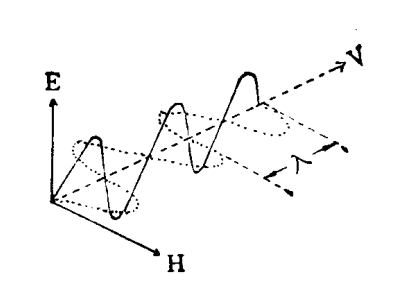
\includegraphics[width=0.7\linewidth]{electromagnetic_wave_structure.png}
    \caption{电磁波传播示意图（电场和磁场互相垂直）}
    \label{fig:electromagnetic_wave_structure}
\end{figure}

交替产生变化的电场和磁场，由近及远地传播，就叫做电磁波。实践证明电场和磁场都具有能量，因此电磁波的传播过程就是能量的传播过程。

\section{传播模式分类}

无线电波在空间中的传播主要有以下几种模式：

\subsection{地波传播}
地波传播是指无线电波沿地球表面传播的方式，适用于低频和中频信号。
\begin{itemize}[leftmargin=3.5em]
    \item \textbf{特点}：信号稳定，受天气影响小，传播距离有限
    \item \textbf{适用频段}：低频（LF）和中频（MF）
    \item \textbf{应用场景}：中波广播、导航系统
    \item \textbf{影响因素}：地面电导率、地形地貌
    \item \textbf{传播损耗}：与频率和距离的平方成正比
\end{itemize}

地波传播是指无线电波沿着地球表面绕射以达到传播的方式。在国内短距离广播主要使用中波，中波主要靠地波传播，传播距离约几百公里。

\begin{figure}[htbp]
    \centering
    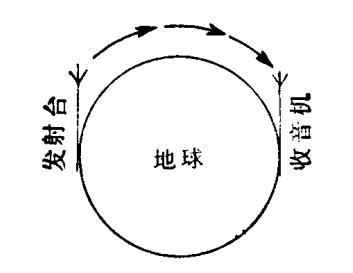
\includegraphics[width=0.7\linewidth]{ground_wave.png}
    \caption{地波传播示意图}
    \label{fig:ground_wave}
\end{figure}

\subsection{天波传播}
天波传播是指无线电波通过电离层反射传播的方式，适用于高频信号。
\begin{itemize}[leftmargin=3.5em]
    \item \textbf{特点}：传播距离远，可以跨越大陆和海洋，信号不稳定
    \item \textbf{适用频段}：高频（HF）
    \item \textbf{应用场景}：短波广播、国际通信
    \item \textbf{影响因素}：电离层变化、太阳活动、昼夜变化
    \item \textbf{最佳工作频率}：通常为最高可用频率的85\%
\end{itemize}

远距离（或国际之间）广播及通讯等都使用短波段。短波段的电波波长比较短，虽然地面对它的吸收很强，只能沿着地球表面大约传几十公里，然而电离层对它的吸收较弱，而且反射角很大。

约离地球六、七十公里至二、三百公里的高空中存在有电离层，短波主要靠它与地面之间的往返反射而形成远距离传播，这种传播方式称为天波传播。天波传播会受季节、昼夜、地理环境、太阳黑子等因素的变化而发生变化，这样就影响了无线电波的传播。

\begin{figure}[htbp]
    \centering
    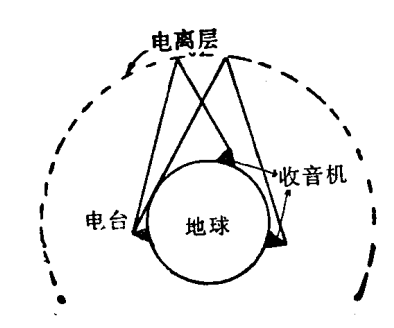
\includegraphics[width=0.7\linewidth]{ionosphere_reflection.png}
    \caption{短波电离层反射示意图}
    \label{fig:ionosphere_reflection}
\end{figure}

\subsection{空间波传播}
空间波传播是指无线电波在空间中直线传播的方式，适用于甚高频和特高频信号。
\begin{itemize}[leftmargin=3.5em]
    \item \textbf{特点}：信号质量好，带宽大，传播距离短
    \item \textbf{适用频段}：甚高频（VHF）和特高频（UHF）
    \item \textbf{应用场景}：调频广播、电视广播、移动通信
    \item \textbf{影响因素}：地球曲率、障碍物遮挡
    \item \textbf{视距计算}：$d = 3.57\sqrt{h}$，其中d为视距（km），h为天线高度（m）
\end{itemize}

\subsection{对流层传播}
对流层传播是指无线电波通过对流层散射传播的方式，适用于超短波。
\begin{itemize}[leftmargin=3.5em]
    \item \textbf{特点}：传播距离较远，受天气影响较大
    \item \textbf{适用频段}：超短波（SHF）
    \item \textbf{应用场景}：远程通信、雷达
    \item \textbf{影响因素}：对流层不稳定度、水汽含量
\end{itemize}

\subsection{卫星传播}
卫星传播是指无线电波通过人造卫星中继传播的方式，适用于全球通信。
\begin{itemize}[leftmargin=3.5em]
    \item \textbf{特点}：覆盖范围广，通信质量稳定
    \item \textbf{适用频段}：微波（SHF、EHF）
    \item \textbf{应用场景}：卫星通信、卫星电视、全球定位系统
    \item \textbf{影响因素}：卫星轨道、大气衰减
    \item \textbf{延迟特性}：地球同步卫星的单程延迟约为270ms
\end{itemize}

\section{传播模型}

无线电波传播模型是预测信号在不同环境中传播特性的数学模型，对于无线通信系统的设计和优化具有重要意义。

\subsection{自由空间传播模型}
自由空间传播是电磁波在理想真空或均匀介质中的传播模型，是最简单的传播模型。

自由空间传播损耗的计算公式为：
\begin{equation}
L = 32.45 + 20\log_{10}(f) + 20\log_{10}(d)
\end{equation}
其中，L为传播损耗（dB），f为频率（MHz），d为距离（km）。

\subsection{地面传播模型}
地面传播模型考虑了地球表面的影响，适用于地波传播和视距传播。
\begin{itemize}[leftmargin=3.5em]
    \item \textbf{Okumura-Hata模型}：适用于城市环境的传播预测
    \item \textbf{COST-231模型}：适用于宏蜂窝系统的传播预测
    \item \textbf{Walfisch-Ikegami模型}：适用于市区微蜂窝系统的传播预测
\end{itemize}

\section{现代传播模型}

\subsection{室内传播模型}
室内传播模型考虑了建筑物内部的环境影响，适用于室内无线通信系统。
\begin{itemize}[leftmargin=3.5em]
    \item \textbf{对数距离路径损耗模型}：$L = L_0 + 10n\log_{10}(d/d_0)$，其中n为路径损耗指数
    \item \textbf{多墙模型}：考虑墙壁和障碍物的影响
    \item \textbf{射线跟踪模型}：基于电磁波传播的物理原理
\end{itemize}

\subsection{毫米波传播模型}
毫米波传播适用于5G/6G通信系统，具有独特的传播特性。
\begin{itemize}[leftmargin=3.5em]
    \item \textbf{高路径损耗}：与频率的平方成正比
    \item \textbf{大气吸收}：在60GHz频段有显著的氧气吸收
    \item \textbf{穿透能力弱}：难以穿透墙壁等障碍物
    \item \textbf{反射特性}：利用反射进行非视距传播
\end{itemize}

\section{传播影响因素与改善措施}

\subsection{主要影响因素}
\begin{itemize}[leftmargin=3.5em]
    \item \textbf{地形地貌}：山脉、建筑物等对信号的遮挡、反射和散射
    \item \textbf{大气条件}：雨、雪、雾等天气条件会对高频无线电波产生衰减
    \item \textbf{电离层变化}：太阳活动、昼夜变化对天波传播的影响
    \item \textbf{电磁干扰}：其他无线电设备、电气设备、自然现象等产生的干扰信号
    \item \textbf{多径效应}：信号通过不同路径到达接收端产生的干扰
\end{itemize}

\subsection{接收效果改善措施}
\begin{itemize}[leftmargin=3.5em]
    \item \textbf{调整天线位置}：选择开阔、无遮挡的位置安装天线
    \item \textbf{使用定向天线}：提高信号接收强度，减少干扰
    \item \textbf{增加信号放大器}：增强弱信号的接收能力
    \item \textbf{采用分集接收}：通过多个天线接收信号，减少多径效应的影响
    \item \textbf{优化接收设备}：使用高性能的接收器和信号处理电路
    \item \textbf{智能天线技术}：使用波束成形技术提高接收质量
\end{itemize}

\chapter{调制技术原理}

本章介绍调制技术的基本原理、分类和应用。调制是将信息信号加载到载波上的关键技术，决定了通信系统的性能。主要内容包括调制基础概念、调制方式分类、模拟调制技术、数字调制技术和现代调制技术。

\section{调制基础概念}

调制是将基带信号加载到高频载波上的过程，是无线电通信的核心技术。调制的主要目的是：

\begin{itemize}[leftmargin=3.5em]
    \item \textbf{频率变换}：将低频信号变换到适合传输的高频
    \item \textbf{频谱搬移}：将信号频谱搬移到指定频段
    \item \textbf{多路复用}：在同一频段内传输多路信号
    \item \textbf{抗干扰}：提高信号在传输过程中的抗干扰能力
    \item \textbf{功率效率}：提高信号的传输效率和功率利用率
\end{itemize}

\section{调制方式分类}

根据调制信号的类型和调制参数的不同，调制可以分为以下几类：

\begin{itemize}[leftmargin=3.5em]
    \item \textbf{模拟调制}：使用模拟信号进行调制，如调幅（AM）、调频（FM）、调相（PM）
    \item \textbf{数字调制}：使用数字信号进行调制，如幅移键控（ASK）、频移键控（FSK）、相移键控（PSK）、正交幅度调制（QAM）
    \item \textbf{混合调制}：结合模拟和数字调制技术的混合调制方式
\end{itemize}

\section{模拟调制技术}

\subsection{调幅（AM）}
调幅是改变载波的振幅，使其随信息信号的变化而变化的调制方式。
\begin{itemize}[leftmargin=3.5em]
    \item \textbf{工作原理}：载波的振幅随调制信号的变化而变化
    \item \textbf{数学表达式}：$s(t) = [A + m(t)]\cos(2\pi f_c t)$，其中$A$为载波振幅，$m(t)$为调制信号
    \item \textbf{优点}：电路简单，成本低，占用频带窄
    \item \textbf{缺点}：抗干扰能力差，音质一般
    \item \textbf{应用场景}：中波广播、短波广播
    \item \textbf{调制指数}：衡量调制深度的参数，通常在0.3-0.8之间
\end{itemize}

\subsection{调频（FM）}
调频是改变载波的频率，使其随信息信号的变化而变化的调制方式。
\begin{itemize}[leftmargin=3.5em]
    \item \textbf{工作原理}：载波的频率随调制信号的变化而变化
    \item \textbf{数学表达式}：$s(t) = A\cos[2\pi f_c t + k_f \int m(\tau)d\tau]$，其中$k_f$为调频灵敏度
    \item \textbf{优点}：抗干扰能力强，音质好
    \item \textbf{缺点}：占用频带宽，电路复杂
    \item \textbf{应用场景}：超短波广播、电视伴音、移动通信
    \item \textbf{调制指数}：衡量频率偏移程度的参数，通常大于1
\end{itemize}

\subsection{调相（PM）}
调相是改变载波的相位，使其随信息信号的变化而变化的调制方式。
\begin{itemize}[leftmargin=3.5em]
    \item \textbf{工作原理}：载波的相位随调制信号的变化而变化
    \item \textbf{数学表达式}：$s(t) = A\cos[2\pi f_c t + k_p m(t)]$，其中$k_p$为调相灵敏度
    \item \textbf{优点}：抗干扰能力强，带宽利用率高
    \item \textbf{缺点}：电路复杂，对相位噪声敏感
    \item \textbf{应用场景}：数字通信、卫星通信
\end{itemize}

\section{数字调制技术}

数字调制是使用数字信号进行调制的方式，具有抗干扰能力强、传输效率高、便于加密等优点。

\subsection{基本数字调制方式}
\begin{itemize}[leftmargin=3.5em]
    \item \textbf{幅移键控（ASK）}：通过改变载波的振幅来传输数字信息
    \item \textbf{频移键控（FSK）}：通过改变载波的频率来传输数字信息
    \item \textbf{相移键控（PSK）}：通过改变载波的相位来传输数字信息
    \item \textbf{正交幅度调制（QAM）}：同时改变载波的振幅和相位来传输数字信息
\end{itemize}

\subsection{高级数字调制技术}
\begin{itemize}[leftmargin=3.5em]
    \item \textbf{正交频分复用（OFDM）}：将高速数据分成多个低速子载波并行传输，提高频谱利用率
    \item \textbf{码分多址（CDMA）}：使用扩频技术实现多用户共享信道
    \item \textbf{正交相移键控（QPSK）}：一种高效的四相调制方式，广泛应用于卫星通信和数字电视
    \item \textbf{16QAM/64QAM}：高阶调制方式，提高频谱利用率，适用于高速数据传输
    \item \textbf{256QAM/1024QAM}：超高阶调制方式，用于5G/6G高速数据传输
    \item \textbf{滤波器组多载波（FBMC）}：OFDM的改进版本，具有更好的频谱特性
\end{itemize}

\section{现代调制技术}

\subsection{5G/6G调制技术}
\begin{itemize}[leftmargin=3.5em]
    \item \textbf{高阶QAM}：256QAM、1024QAM等，提高频谱效率
    \item \textbf{非正交多址（NOMA）}：允许多用户在同一资源块上传输
    \item \textbf{全双工通信}：在同一频率上同时收发信号
    \item \textbf{太赫兹调制}：针对太赫兹频段的特殊调制技术
\end{itemize}

\subsection{毫米波调制技术}
\begin{itemize}[leftmargin=3.5em]
    \item \textbf{混合波束成形}：结合数字和模拟波束成形
    \item \textbf{压缩感知}：减少毫米波系统的反馈开销
    \item \textbf{空间调制}：利用天线索引传递信息
\end{itemize}

\section{练习与思考}

1. 什么是调制？调制的主要目的是什么？
2. 调制的基本类型有哪些？它们的特点是什么？
3. 模拟调制和数字调制的区别是什么？
4. AM调制和FM调制的工作原理是什么？它们的优缺点是什么？
5. 数字调制的基本方式有哪些？它们的误码率性能如何？
6. QPSK调制的工作原理是什么？它的频谱效率是多少？
7. 高阶QAM调制的优缺点是什么？
8. OFDM技术的工作原理是什么？它在5G通信中的应用是什么？
9. 非正交多址（NOMA）技术的优势是什么？
10. 毫米波调制技术的特点是什么？

\chapter{传播与调制应用}
\label{传播与调制应用}

关于调制技术在实际应用中的具体案例，请参考本章内容。

\section{典型应用场景}

\subsection{广播系统}
\begin{itemize}[leftmargin=3.5em]
    \item \textbf{中波广播}：使用AM调制，覆盖范围广
    \item \textbf{调频广播}：使用FM调制，音质好
    \item \textbf{数字广播}：使用DAB/DAB+，音质更好，抗干扰能力强
\end{itemize}

\subsection{移动通信系统}
\begin{itemize}[leftmargin=3.5em]
    \item \textbf{2G系统}：使用GMSK调制，频谱效率较低
    \item \textbf{3G系统}：使用QPSK/16QAM调制，支持数据业务
    \item \textbf{4G系统}：使用OFDM调制，频谱效率显著提高
    \item \textbf{5G系统}：使用高阶QAM和OFDM，支持超高速数据传输
    \item \textbf{6G系统}：探索太赫兹通信和智能表面技术
\end{itemize}

\subsection{卫星通信系统}
\begin{itemize}[leftmargin=3.5em]
    \item \textbf{固定卫星服务}：使用QPSK/8PSK调制
    \item \textbf{移动卫星服务}：使用高效调制方式，适应移动环境
    \item \textbf{卫星互联网}：使用波束成形和高效调制技术
\end{itemize}

\subsection{无线局域网}
\begin{itemize}[leftmargin=3.5em]
    \item \textbf{Wi-Fi 5}：使用OFDM调制，最高速率3.5Gbps
    \item \textbf{Wi-Fi 6}：使用1024QAM和MU-MIMO，最高速率9.6Gbps
    \item \textbf{Wi-Fi 7}：使用4096QAM和多链路操作，最高速率30Gbps
\end{itemize}

\section{调制方式选择指南}

选择合适的调制方式需要考虑以下因素：
\begin{itemize}[leftmargin=3.5em]
    \item \textbf{信道条件}：根据信道质量选择合适的调制阶数
    \item \textbf{传输速率}：高速传输需要高阶调制
    \item \textbf{抗干扰能力}：恶劣环境需要更鲁棒的调制方式
    \item \textbf{功率效率}：功率受限场景需要功率效率高的调制方式
    \item \textbf{复杂度}：考虑硬件实现的复杂度和成本
\end{itemize}

\section{传播预测与系统设计}

\subsection{传播预测工具}
\begin{itemize}[leftmargin=3.5em]
    \item \textbf{Okumura-Hata模型}：适用于城市环境的传播预测
    \item \textbf{COST-231模型}：适用于宏蜂窝系统的传播预测
    \item \textbf{射线跟踪工具}：如Remcom Wireless InSite、WinProp等
\end{itemize}

\subsection{系统设计流程}
\begin{itemize}[leftmargin=3.5em]
    \item \textbf{需求分析}：确定系统的覆盖范围、容量和服务质量要求
    \item \textbf{传播预测}：使用合适的模型预测信号传播特性
    \item \textbf{调制选择}：根据信道条件选择合适的调制方式
    \item \textbf{天线设计}：根据传播特性设计合适的天线系统
    \item \textbf{系统仿真}：使用仿真工具验证系统性能
    \item \textbf{现场测试}：实际测试系统性能，进行优化
\end{itemize}

\section{总结与展望}

无线电波传播与调制技术是无线通信系统的核心组成部分。随着5G/6G、毫米波通信、太赫兹通信等新技术的发展，传播与调制技术也在不断演进。未来的发展方向包括：

\begin{itemize}[leftmargin=3.5em]
    \item \textbf{智能传播预测}：利用人工智能技术提高传播预测的准确性
    \item \textbf{自适应调制}：根据信道条件自动调整调制方式
    \item \textbf{超高频段调制}：针对太赫兹等超高频段的调制技术
    \item \textbf{绿色调制}：低功耗、高效率的调制技术
    \item \textbf{一体化设计}：传播与调制的联合优化设计
\end{itemize}

了解并掌握这些技术，对于设计和优化现代无线通信系统具有重要意义。

\part{无线电技术基础}

\chapter{电源系统}

本章介绍无线电设备的电源系统设计，包括电源类型选择、整流电路、滤波电路和稳压技术。电源系统是无线电设备稳定运行的基础。主要内容包括电源类型与选择、整流电路、滤波电路、稳压电路、电源保护电路和现代电源技术。

\section{电源类型与选择}

电源系统是无线电设备的重要组成部分，为设备提供稳定的工作电源。电源类型根据供电方式的不同，可以分为交流电源、直流电源、电池电源、太阳能电源等。

\subsection{交流电源}

交流电源是指使用市电（220V或110V交流电）供电的电源系统。交流电源的优点是功率大、稳定性好、成本低；缺点是需要电源适配器，便携性差。交流电源主要用于家用无线电设备、固定台站等功率需求较大的设备。

交流电源系统通常包括：
\begin{itemize}
    \item 电源插座和电源线
    \item 电源适配器（AC-DC转换器）
    \item 浪涌保护电路
    \item 电磁兼容（EMC）滤波电路
\end{itemize}

\subsection{直流电源}

直流电源是指使用直流电供电的电源系统，通常通过电源适配器将交流电转换为直流电，或直接使用直流电源。直流电源的优点是稳定性好、纹波小；缺点是需要电源适配器，便携性差。直流电源主要用于家用无线电设备、车载无线电设备和固定台站。

常见的直流电源规格包括：
\begin{itemize}
    \item 5V：适用于低功耗设备，如便携式收音机
    \item 12V：适用于中等功率设备，如车载电台
    \item 24V：适用于大功率设备，如基站设备
\end{itemize}

\subsection{电池电源}

电池电源是指使用电池供电的电源系统。电池电源的优点是便携性好、使用方便；缺点是功率小、需要定期更换或充电。电池电源主要用于便携无线电设备、车载无线电设备和应急通信设备。

\subsubsection{电池类型对比}

\begin{tabular}{|l|l|l|l|l|}
\hline
电池类型 & 优点 & 缺点 & 典型电压 & 适用设备 \\
\hline
锂电池 & 能量密度高、循环寿命长 & 成本高、需要保护电路 & 3.7V & 智能手机、便携电台 \\
\hline
镍氢电池 & 安全、环保、无记忆效应 & 能量密度较低、自放电率高 & 1.2V & 手持对讲机 \\
\hline
锂聚合物电池 & 形状灵活、能量密度高 & 成本高、寿命较短 & 3.7V & 超薄设备、无人机 \\
\hline
燃料电池 & 能量密度极高、环保 & 成本高、系统复杂 & 多种电压 & 应急通信、远程设备 \\
\hline
\end{tabular}

\subsubsection{电池管理系统（BMS）}

电池管理系统是电池电源的核心组成部分，主要功能包括：
\begin{itemize}
    \item 电池状态监测（SOC、SOH）
    \item 充放电保护
    \item 温度管理
    \item 均衡充电
    \item 电量显示
\end{itemize}

\subsection{太阳能电源}

太阳能电源是指使用太阳能电池板供电的电源系统。太阳能电源的优点是环保、可持续；缺点是功率小、受天气影响大。太阳能电源主要用于户外无线电设备、应急无线电设备和远程监测站。

太阳能电源系统通常包括：
\begin{itemize}
    \item 太阳能电池板
    \item 充电控制器
    \item 储能电池
    \item 逆变器（AC输出时）
\end{itemize}

\subsection{电源管理IC（PMIC）}

电源管理IC是现代电源系统的核心组件，集成了多种功能：
\begin{itemize}
    \item 电压调节
    \item 电流控制
    \item 功率管理
    \item 电池充电
    \item 保护功能
\end{itemize}

常见的电源管理IC厂商包括TI、Maxim、Linear Technology等。

\subsection{电源选择指南}

选择合适的电源类型，需要考虑以下因素：

\begin{itemize}
    \item \textbf{使用场景}：家用、车载、便携、户外等
    \item \textbf{功率需求}：低功耗（<1W）、中等功率（1-50W）、大功率（>50W）
    \item \textbf{便携性要求}：固定安装、移动使用、手持设备
    \item \textbf{环境条件}：温度范围、湿度、振动等
    \item \textbf{可靠性要求}：工业级、商业级、消费级
    \item \textbf{成本预算}：高端、中端、经济型
\end{itemize}

\subsubsection{电源选择流程图}

\begin{enumerate}
    \item 确定设备功率需求
    \item 确定使用场景和环境条件
    \item 评估便携性要求
    \item 选择电源类型（交流、直流、电池、太阳能）
    \item 确定具体电源规格和保护电路
    \item 验证电源系统的可靠性和安全性
\end{enumerate}

\section{整流电路}

整流电路是将交流电转换为直流电的电路，是直流电源的重要组成部分。整流的基本原理是利用二极管的单向导电性，将交流电转换为脉动直流电。

\subsection{半波整流}

半波整流是最简单的整流电路，只利用交流电的正半周或负半周，效率低，纹波大。

\subsubsection{电路原理}

半波整流电路由一个二极管和负载组成。当交流电压为正时，二极管导通，电流流向负载；当交流电压为负时，二极管截止，无电流通过。

\subsubsection{计算公式}

\begin{itemize}
    \item 输出电压平均值：$V_{dc} = \frac{V_{m}}{\pi} \approx 0.318 V_{m}$
    \item 纹波系数：$\gamma = \sqrt{\left(\frac{V_{rms}}{V_{dc}}\right)^2 - 1} \approx 1.21$
    \item 整流效率：$\eta = \frac{P_{dc}}{P_{ac}} \approx 40.6\%$
\end{itemize}

其中，$V_{m}$是交流电压的峰值。

\subsection{全波整流}

全波整流利用交流电的正半周和负半周，效率较高，纹波较小。

\subsubsection{电路原理}

全波整流电路通常使用两个二极管和一个中心抽头变压器。正负半周都有电流通过负载，提高了整流效率。

\subsubsection{计算公式}

\begin{itemize}
    \item 输出电压平均值：$V_{dc} = \frac{2V_{m}}{\pi} \approx 0.636 V_{m}$
    \item 纹波系数：$\gamma \approx 0.483$
    \item 整流效率：$\eta \approx 81.2\%$
\end{itemize}

\subsection{桥式整流}

桥式整流是全波整流的一种，使用四个二极管组成桥式电路，效率高，纹波小，广泛应用于各种整流电路中。

\subsubsection{电路原理}

桥式整流电路由四个二极管组成，不需要中心抽头变压器，能够利用交流电的正负半周，输出脉动直流电。

\subsubsection{计算公式}

\begin{itemize}
    \item 输出电压平均值：$V_{dc} = \frac{2V_{m}}{\pi} \approx 0.636 V_{m}$
    \item 纹波系数：$\gamma \approx 0.483$
    \item 整流效率：$\eta \approx 81.2\%$
\end{itemize}
\begin{itemize}
    \item 二极管反向电压：$V_{rm} = V_{m}$
\end{itemize}

\subsection{整流电路参数对比}

\begin{tabular}{|l|l|l|l|l|}
\hline
整流类型 & 输出电压 & 纹波系数 & 整流效率 & 二极管数量 \\
\hline
半波整流 & $0.318 V_{m}$ & 1.21 & 40.6\% & 1 \\
\hline
全波整流 & $0.636 V_{m}$ & 0.483 & 81.2\% & 2 \\
\hline
桥式整流 & $0.636 V_{m}$ & 0.483 & 81.2\% & 4 \\
\hline
\end{tabular}

\subsection{整流电路设计实例}

\subsubsection{12V直流电源整流电路设计}

\textbf{设计参数：}
\begin{itemize}
    \item 输入电压：AC 220V/50Hz
    \item 输出电压：DC 12V
    \item 输出电流：1A
\end{itemize}

\textbf{设计步骤：}

\begin{enumerate}
    \item \textbf{变压器选择：}
    \begin{itemize}
        \item 输出电压：$V_{ac} = \frac{V_{dc}}{0.9} = \frac{12V}{0.9} \approx 13.3V$
        \item 变压器功率：$P = V_{dc} \times I_{dc} = 12V \times 1A = 12W$
        \item 选择15V/1A变压器
    \end{itemize}

    \item \textbf{整流桥选择：}
    \begin{itemize}
        \item 峰值电压：$V_{m} = \sqrt{2} \times 15V \approx 21.2V$
        \item 反向电压：$V_{rm} = 21.2V$
        \item 选择1A/50V整流桥
    \end{itemize}

    \item \textbf{滤波电容选择：}
    \begin{itemize}
        \item 电容值：$C = \frac{I_{dc} \times t}{\Delta V}$
        \item 取$t = 10ms$（50Hz半周期），$\Delta V = 1V$
        \item $C = \frac{1A \times 0.01s}{1V} = 0.01F = 10000\mu F$
    \end{itemize}

    \item \textbf{保护电路：}
    \begin{itemize}
        \item 保险丝：2A
        \item 压敏电阻：275V
    \end{itemize}
\end{enumerate}

\textbf{电路图：}

\begin{verbatim}
[变压器] → [整流桥] → [滤波电容] → [稳压电路] → [负载]
\end{verbatim}

\subsubsection{整流桥芯片推荐}

\begin{itemize}
    \item \textbf{KBPC系列}：KBPC1010（10A/1000V），适用于大功率设备
    \item \textbf{MB6S系列}：MB6S（0.5A/600V），适用于小功率设备
    \item \textbf{GBJ系列}：GBJ2510（25A/1000V），适用于工业设备
\end{itemize}

\subsection{功率因数校正（PFC）}

功率因数校正是提高电源效率的重要技术，主要分为：

\begin{itemize}
    \item \textbf{无源PFC}：使用电感和电容组成的滤波电路
    \item \textbf{有源PFC}：使用开关电路主动调整输入电流
\end{itemize}

有源PFC的功率因数可达到0.99以上，显著减少谐波干扰。

\section{滤波电路}

滤波电路是滤除整流后脉动直流电中的交流成分，使输出电压更加平滑的电路。滤波的基本原理是利用电容、电感等元件的储能特性，平滑输出电压。

\subsection{电容滤波}

电容滤波是最简单的滤波电路，通过电容的充放电平滑输出电压，结构简单，成本低，但滤波效果一般。

\subsubsection{电路原理}

电容滤波电路由一个电解电容并联在负载两端组成。当整流输出电压高于电容电压时，电容充电；当整流输出电压低于电容电压时，电容放电，从而平滑输出电压。

\subsubsection{计算公式}

\begin{itemize}
    \item 纹波电压：$V_{r} \approx \frac{I_{dc}}{2fC}$
    \item 电容容量：$C \approx \frac{I_{dc}}{2fV_{r}}$
\end{itemize}

其中，$f$是交流电源频率，$I_{dc}$是直流输出电流，$V_{r}$是允许的纹波电压。

\subsection{电感滤波}

电感滤波通过电感的储能特性平滑输出电压，滤波效果较好，但体积大，成本高。

\subsubsection{电路原理}

电感滤波电路由一个电感串联在整流输出和负载之间。电感对交流成分呈现高阻抗，对直流成分呈现低阻抗，从而滤除交流纹波。

\subsubsection{计算公式}

\begin{itemize}
    \item 纹波系数：$\gamma \approx \frac{R_{L}}{3\omega L}$
    \item 电感值：$L \approx \frac{R_{L}}{3\omega \gamma}$
\end{itemize}

其中，$R_{L}$是负载电阻，$\omega = 2\pi f$是角频率，$\gamma$是允许的纹波系数。

\subsection{LC滤波与π型滤波}

LC滤波结合了电容滤波和电感滤波的优点，滤波效果好，广泛应用于各种滤波电路中。π型滤波由两个电容和一个电感组成，滤波效果最好，但电路复杂，成本高。

\subsubsection{LC滤波}

LC滤波电路由一个电感和一个电容组成，形成低通滤波器，能够有效滤除高频纹波。

\subsubsection{π型滤波}

π型滤波电路由两个电容和一个电感组成，形成π型结构，滤波效果优于LC滤波，适用于对纹波要求较高的场合。

\subsection{滤波电路参数对比}

\begin{tabular}{|l|l|l|l|l|l|}
\hline
滤波类型 & 滤波效果 & 成本 & 体积 & 适用场合 & 纹波系数 \\
\hline
电容滤波 & 一般 & 低 & 小 & 小功率设备 & 较大 \\
\hline
电感滤波 & 较好 & 中 & 大 & 中功率设备 & 中等 \\
\hline
LC滤波 & 好 & 中 & 中 & 中大功率设备 & 较小 \\
\hline
π型滤波 & 最好 & 高 & 大 & 精密设备 & 很小 \\
\hline
\end{tabular}

\subsection{EMI滤波设计}

电磁干扰（EMI）滤波是现代电源设计的重要组成部分，主要包括：

\subsubsection{差模滤波}
\begin{itemize}
    \item 使用差模电感和电容
    \item 滤除相线和中线之间的干扰
\end{itemize}

\subsubsection{共模滤波}
\begin{itemize}
    \item 使用共模电感和Y电容
    \item 滤除相线和地线之间的干扰
\end{itemize}

\subsubsection{EMI滤波器设计要点}
\begin{itemize}
    \item 选择合适的滤波元件值
    \item 合理布局，减少寄生参数
    \item 屏蔽设计，防止辐射干扰
\end{itemize}

\subsection{滤波电路频率响应}

不同滤波电路的频率响应特性：

\begin{itemize}
    \item \textbf{电容滤波}：低通特性，截止频率$f_{c} = \frac{1}{2\pi R_{L}C}$
    \item \textbf{电感滤波}：低通特性，截止频率$f_{c} = \frac{R_{L}}{2\pi L}$
    \item \textbf{LC滤波}：二阶低通，截止频率$f_{c} = \frac{1}{2\pi \sqrt{LC}}$
    \item \textbf{π型滤波}：三阶低通，滤波效果更好
\end{itemize}

\subsection{滤波电路设计实例}

\subsubsection{12V/1A电源滤波电路设计}

\textbf{设计参数：}
\begin{itemize}
    \item 输入电压：DC 15V（整流后）
    \item 输出电压：DC 12V
    \item 输出电流：1A
    \item 纹波要求：$\leq 100mV_{pp}$
\end{itemize}

\textbf{设计步骤：}

\begin{enumerate}
    \item \textbf{电容滤波设计：}
    \begin{itemize}
        \item 计算电容值：$C = \frac{I_{dc}}{2fV_{r}} = \frac{1A}{2 \times 50Hz \times 0.1V} = 10000\mu F$
        \item 选择10000μF/25V电解电容
    \end{itemize}

    \item \textbf{LC滤波设计：}
    \begin{itemize}
        \item 电感值：$L = \frac{R_{L}}{3\omega \gamma}$，取$\gamma = 0.01$
        \item $R_{L} = \frac{12V}{1A} = 12\Omega$
        \item $L = \frac{12}{3 \times 314 \times 0.01} \approx 12.7mH$
        \item 选择15mH电感
    \end{itemize}

    \item \textbf{π型滤波设计：}
    \begin{itemize}
        \item 输入电容：10000μF
        \item 电感：15mH
        \item 输出电容：2200μF
    \end{itemize}
\end{enumerate}

\textbf{电路图：}

\begin{verbatim}
[整流输出] → [C1:10000μF] → [L:15mH] → [C2:2200μF] → [负载]
\end{verbatim}

\subsubsection{EMI滤波器设计}

\textbf{设计参数：}
\begin{itemize}
    \item 输入电压：AC 220V/50Hz
    \item 输出功率：12W
    \item EMI标准：EN 55022 Class B
\end{itemize}

\textbf{设计方案：}
\begin{itemize}
    \item 共模电感：10mH
    \item 差模电感：1mH
    \item X电容：0.1μF
    \item Y电容：2200pF
\end{itemize}

\textbf{电路图：}

\begin{verbatim}
[输入] → [共模电感] → [X电容] → [差模电感] → [整流桥]
\end{verbatim}

\subsection{滤波电路PCB布局技巧}

\begin{enumerate}
    \item \textbf{元件布局：}
    \begin{itemize}
        \item 滤波电容靠近整流输出
        \item 电感远离敏感电路
        \item 地线回路尽量短
    \end{itemize}

    \item \textbf{布线注意事项：}
    \begin{itemize}
        \item 大电流回路避免与小信号回路交叉
        \item 输入输出线分开布线
        \item 使用地线平面，减少EMI
    \end{itemize}

    \item \textbf{散热设计：}
    \begin{itemize}
        \item 电感和电容的散热考虑
        \item 避免热元件靠近电解电容
    \end{itemize}
\end{enumerate}

滤波电路的设计需要考虑纹波系数、输出电压稳定性、滤波效率、体积成本等多种因素。好的滤波电路能够在满足纹波系数和稳定性要求的同时，保持高滤波效率和低体积成本。

\section{稳压电路}

稳压电路是保持输出电压稳定的电路，是电源系统的重要组成部分。稳压的基本原理是通过负反馈控制，使输出电压保持稳定，不受输入电压变化和负载变化的影响。

\subsection{线性稳压}

线性稳压通过调整管的线性调节，使输出电压保持稳定，具有结构简单、纹波小的优点，但效率低，功耗大。

\subsubsection{工作原理}

线性稳压器的基本结构包括：
\begin{itemize}
    \item 参考电压源
    \item 误差放大器
    \item 调整管
    \item 反馈网络
\end{itemize}

当输入电压或负载变化时，误差放大器检测输出电压的变化，通过调整管的导通程度来保持输出电压稳定。

\subsubsection{常用线性稳压芯片}

\begin{tabular}{|l|l|l|l|l|l|}
\hline
芯片型号 & 输出电压 & 输出电流 & 输入电压范围 & 纹波抑制比 & 封装 \\
\hline
7805 & 5V & 1A & 7-20V & 68dB & TO-220 \\
\hline
7812 & 12V & 1A & 14-27V & 68dB & TO-220 \\
\hline
LM317 & 1.2-37V & 1.5A & 3-40V & 80dB & TO-220 \\
\hline
LM1117 & 1.8-5V & 800mA & 2.5-15V & 60dB & SOT-223 \\
\hline
LT1083 & 1.25-30V & 7.5A & 2.5-35V & 80dB & TO-3 \\
\hline
\end{tabular}

\subsection{开关稳压}

开关稳压通过调整管的开关调节，使输出电压保持稳定，具有效率高、功耗小的优点，但电路复杂，纹波较大。

\subsubsection{工作原理}

开关稳压器的基本结构包括：
\begin{itemize}
    \item 开关管
    \item 电感和电容
    \item 控制电路
    \item 反馈网络
\end{itemize}

通过控制开关管的导通和截止时间，将输入电压转换为脉冲信号，再通过电感和电容滤波得到稳定的直流输出。

\subsubsection{常用开关稳压芯片}

\begin{tabular}{|l|l|l|l|l|l|}
\hline
芯片型号 & 拓扑结构 & 输出电压 & 输出电流 & 效率 & 开关频率 \\
\hline
LM2596 & Buck & 3.3/5/12V & 3A & 75-88\% & 150kHz \\
\hline
LM2576 & Buck & 3.3/5/12V & 3A & 75-88\% & 52kHz \\
\hline
MP2307 & Buck & 0.8-24V & 3A & 92\% & 2.5MHz \\
\hline
XL6009 & Boost & 5-35V & 4A & 88\% & 300kHz \\
\hline
LM2577 & Buck-Boost & 1.25-37V & 3A & 75\% & 52kHz \\
\hline
\end{tabular}

\subsection{线性稳压器与开关稳压器对比}

\begin{tabular}{|l|l|l|}
\hline
特性 & 线性稳压器 & 开关稳压器 \\
\hline
效率 & 低（40-60\%） & 高（75-95\%） \\
\hline
纹波 & 小（<1mV） & 大（10-100mV） \\
\hline
成本 & 低 & 高 \\
\hline
体积 & 小 & 大（需电感） \\
\hline
EMI & 小 & 大 \\
\hline
散热 & 差（需 heatsink） & 好 \\
\hline
响应速度 & 快 & 慢 \\
\hline
适用场合 & 小功率、低纹波 & 大功率、高效率 \\
\hline
\end{tabular}

\subsection{稳压二极管}

稳压二极管利用稳压二极管的反向击穿特性，使输出电压保持稳定，具有结构简单、成本低的优点，但稳压精度低，功率小。

\subsubsection{工作原理}

当反向电压达到稳压二极管的击穿电压时，二极管进入击穿状态，电流在很大范围内变化时，电压保持基本稳定。

\subsubsection{常用稳压二极管}

\begin{tabular}{|l|l|l|l|}
\hline
型号 & 稳压值 & 功率 & 误差范围 \\
\hline
1N4728 & 3.3V & 1W & $\pm$5\% \\
\hline
1N4733 & 5.1V & 1W & $\pm$5\% \\
\hline
1N4742 & 12V & 1W & $\pm$5\% \\
\hline
1N4749 & 24V & 1W & $\pm$5\% \\
\hline
\end{tabular}

\subsection{电压参考源电路}

电压参考源是稳压电路的核心，提供稳定的参考电压。常用的电压参考源包括：

\subsubsection{带隙参考源}
\begin{itemize}
    \item 利用半导体的带隙特性，提供温度稳定的参考电压
    \item 典型值为1.25V
    \item 温度系数低（<10ppm/°C）
\end{itemize}

\subsubsection{齐纳参考源}
\begin{itemize}
    \item 利用齐纳二极管的击穿特性
    \item 电压范围宽（2.4V-200V）
    \item 温度系数中等（50-100ppm/°C）
\end{itemize}

\subsubsection{常用电压参考芯片}

\begin{itemize}
    \item \textbf{LM4040}：1.24V-10V，高精度，低温度系数
    \item \textbf{REF5025}：2.5V，高精度，低噪声
    \item \textbf{ADR4525}：2.5V，超高精度，超低温度系数
\end{itemize}

\subsection{稳压电路重要参数}

稳压电路的重要参数包括稳压精度、输出电流、纹波系数、效率、稳定性等。稳压精度是指稳压电路输出电压的精度，稳压精度越高，无线电设备的性能越稳定。输出电流是指稳压电路能够输出的最大电流，输出电流越大，能够驱动的负载越大。纹波系数是指稳压电路输出电压中的交流成分，纹波系数越小，输出电压越稳定。效率是指稳压电路输出功率与输入功率的比值，效率越高，功耗越低。稳定性是指稳压电路输出电压的稳定性，稳定性越高，无线电设备的性能越稳定。

\subsection{稳压电路选择指南}

选择稳压电路时，需要考虑以下因素：

\subsubsection{根据功率需求选择}
\begin{itemize}
    \item 小功率（<1W）：线性稳压器
    \item 中等功率（1-10W）：线性稳压器或开关稳压器
    \item 大功率（>10W）：开关稳压器
\end{itemize}

\subsubsection{根据纹波要求选择}
\begin{itemize}
    \item 低纹波（<1mV）：线性稳压器
    \item 中等纹波（1-10mV）：线性稳压器或低纹波开关稳压器
    \item 高纹波（>10mV）：开关稳压器
\end{itemize}

\subsubsection{根据效率要求选择}
\begin{itemize}
    \item 高效率要求：开关稳压器
    \item 一般效率要求：线性稳压器
\end{itemize}

\subsubsection{根据成本要求选择}
\begin{itemize}
    \item 低成本：线性稳压器
    \item 中等成本：集成开关稳压器
    \item 高成本：定制开关电源
\end{itemize}

\subsection{稳压电路设计实例}

\subsubsection{5V/1A线性稳压电源设计}

\textbf{设计参数：}
\begin{itemize}
    \item 输入电压：7-12V
    \item 输出电压：5V
    \item 输出电流：1A
    \item 纹波要求：<1mV
\end{itemize}

\textbf{设计方案：}
\begin{itemize}
    \item 选择7805稳压器
    \item 输入电容：10μF
    \item 输出电容：10μF
    \item 散热片：TO-220散热片
\end{itemize}

\textbf{电路图：}

\begin{verbatim}
[输入] → [C1:10μF] → [7805] → [C2:10μF] → [负载]
\end{verbatim}

\subsubsection{12V/2A开关稳压电源设计}

\textbf{设计参数：}
\begin{itemize}
    \item 输入电压：15-24V
    \item 输出电压：12V
    \item 输出电流：2A
    \item 效率要求：>80%
\end{itemize}

\textbf{设计方案：}
\begin{itemize}
    \item 选择LM2596-12
    \item 电感：100μH
    \item 输出电容：1000μF
    \item 续流二极管：1N5822
\end{itemize}

\textbf{电路图：}

\begin{verbatim}
[输入] → [LM2596] → [L:100μH] → [D:1N5822] → [C:1000μF] → [负载]
\end{verbatim}

稳压电路的设计需要考虑稳压精度、输出电流、纹波系数、效率、稳定性等多种因素。好的稳压电路能够在满足稳压精度和输出电流要求的同时，保持低纹波系数、高效率和高稳定性。

\section{电源保护电路}

电源保护电路是电源系统的重要组成部分，能够保护电源和负载设备免受各种异常情况的损害。

\subsection{过流保护}

过流保护电路用于防止电源输出电流超过额定值，保护电源和负载设备安全。常用的过流保护方式包括熔断器保护、电子限流保护、自恢复保险丝等。

\subsubsection{熔断器保护}
\begin{itemize}
    \item \textbf{工作原理}：当电流超过额定值时，熔断器熔断，切断电路
    \item \textbf{优点}：结构简单，成本低
    \item \textbf{缺点}：一次性使用，需要更换
    \item \textbf{选型指南}：选择额定电流为负载电流的1.2-1.5倍
\end{itemize}

\subsubsection{电子限流保护}
\begin{itemize}
    \item \textbf{工作原理}：通过检测电流，当超过阈值时限制输出电流
    \item \textbf{优点}：可重复使用，响应速度快
    \item \textbf{缺点}：电路复杂，成本高
    \item \textbf{典型电路}：使用电流检测电阻和比较器
\end{itemize}

\subsubsection{自恢复保险丝}
\begin{itemize}
    \item \textbf{工作原理}：当电流超过额定值时，电阻急剧增加，限制电流
    \item \textbf{优点}：可自动恢复，无需更换
    \item \textbf{缺点}：响应速度较慢，成本较高
    \item \textbf{选型指南}：选择保持电流为负载电流的1.5-2倍
\end{itemize}

\subsection{过压保护}

过压保护电路用于防止电源输出电压超过额定值，保护负载设备安全。常用的过压保护方式包括稳压二极管钳位、过压保护芯片、可控硅保护等。

\subsubsection{稳压二极管钳位}
\begin{itemize}
    \item \textbf{工作原理}：当电压超过稳压值时，稳压二极管导通，钳位电压
    \item \textbf{优点}：结构简单，成本低
    \item \textbf{缺点}：功率较小，响应速度较慢
    \item \textbf{选型指南}：选择稳压值为额定电压的1.1-1.2倍
\end{itemize}

\subsubsection{过压保护芯片}
\begin{itemize}
    \item \textbf{工作原理}：专用芯片检测电压，超过阈值时切断电路
    \item \textbf{优点}：精度高，响应速度快
    \item \textbf{缺点}：成本较高
    \item \textbf{典型芯片}：LM431、TL431
\end{itemize}

\subsubsection{可控硅保护}
\begin{itemize}
    \item \textbf{工作原理}：过压时触发可控硅导通，短路保护
    \item \textbf{优点}：功率大，响应速度快
    \item \textbf{缺点}：需要额外的触发电路
    \item \textbf{适用场合}：大功率设备
\end{itemize}

\subsection{反接保护}

反接保护电路用于防止电源极性接反时损坏设备。常用的反接保护方式包括二极管串联保护、MOSFET反向保护等。

\subsubsection{二极管串联保护}
\begin{itemize}
    \item \textbf{工作原理}：二极管正向导通，反向截止
    \item \textbf{优点}：结构简单，成本低
    \item \textbf{缺点}：有压降，功耗大
    \item \textbf{选型指南}：选择正向电流为负载电流的2-3倍
\end{itemize}

\subsubsection{MOSFET反向保护}
\begin{itemize}
    \item \textbf{工作原理}：利用MOSFET的体二极管和栅极控制
    \item \textbf{优点}：压降小，功耗低
    \item \textbf{缺点}：电路复杂，成本高
    \item \textbf{选型指南}：选择Rds(on)小的MOSFET
\end{itemize}

\subsection{过温保护}

过温保护电路用于防止电源温度过高造成损坏。常用的过温保护方式包括热敏电阻检测、温度开关保护、芯片内部过温保护等。

\subsubsection{热敏电阻保护}
\begin{itemize}
    \item \textbf{工作原理}：利用NTC热敏电阻的阻值随温度变化
    \item \textbf{优点}：成本低，灵敏度高
    \item \textbf{缺点}：需要校准，线性度差
    \item \textbf{选型指南}：
    \begin{itemize}
        \item 选择合适的B值（3000-4000K）
        \item 选择合适的阻值（25°C时）
        \item 考虑安装位置和热响应时间
    \end{itemize}
\end{itemize}

\subsubsection{温度开关保护}
\begin{itemize}
    \item \textbf{工作原理}：达到设定温度时断开或闭合
    \item \textbf{优点}：结构简单，无需外部电路
    \item \textbf{缺点}：精度较低，重复性差
    \item \textbf{选型指南}：选择动作温度为工作温度的1.2-1.3倍
\end{itemize}

\subsubsection{芯片内部过温保护}
\begin{itemize}
    \item \textbf{工作原理}：集成在芯片内部的温度传感器
    \item \textbf{优点}：集成度高，响应速度快
    \item \textbf{缺点}：不可调节，依赖芯片特性
    \item \textbf{适用场合}：使用集成电源管理芯片
\end{itemize}

\subsection{浪涌保护}

浪涌保护电路用于防止雷击、电网波动等引起的电压浪涌。

\subsubsection{压敏电阻保护}
\begin{itemize}
    \item \textbf{工作原理}：电压超过阈值时电阻急剧下降
    \item \textbf{优点}：响应速度快，成本低
    \item \textbf{缺点}：有寿命限制，不能多次触发
    \item \textbf{选型指南}：选择压敏电压为工作电压的2-2.5倍
\end{itemize}

\subsubsection{TVS二极管保护}
\begin{itemize}
    \item \textbf{工作原理}：瞬态电压抑制二极管
    \item \textbf{优点}：响应速度快， clamping电压准确
    \item \textbf{缺点}：功率较小，成本较高
    \item \textbf{选型指南}：选择击穿电压为工作电压的1.3-1.5倍
\end{itemize}

\subsubsection{气体放电管保护}
\begin{itemize}
    \item \textbf{工作原理}：气体电离导通，分流浪涌电流
    \item \textbf{优点}：功率大，寿命长
    \item \textbf{缺点}：响应速度较慢，有续流
    \item \textbf{适用场合}：雷击保护
\end{itemize}

\subsection{完整的电源保护电路设计}

\subsubsection{12V/2A电源保护电路设计}

\textbf{设计参数：}
\begin{itemize}
    \item 输入电压：15-24V
    \item 输出电压：12V
    \item 输出电流：2A
    \item 保护要求：过流、过压、反接、过温
\end{itemize}

\textbf{设计方案：}

\begin{enumerate}
    \item \textbf{反接保护}：
    \begin{itemize}
        \item 使用MOSFET反向保护电路
        \item 选择IRF3205 MOSFET
    \end{itemize}
    
    \item \textbf{过流保护}：
    \begin{itemize}
        \item 使用电流检测电阻+比较器
        \item 检测电阻：0.1Ω
        \item 比较器：LM393
    \end{itemize}
    
    \item \textbf{过压保护}：
    \begin{itemize}
        \item 使用TL431+可控硅
        \item 保护电压：15V
    \end{itemize}
    
    \item \textbf{过温保护}：
    \begin{itemize}
        \item 使用NTC热敏电阻
        \item 动作温度：85°C
    \end{itemize}
    
    \item \textbf{浪涌保护}：
    \begin{itemize}
        \item 压敏电阻：275V
        \item TVS二极管：18V
    \end{itemize}
\end{enumerate}

\textbf{电路图：}

\begin{verbatim}
[输入] → [压敏电阻] → [反接保护MOSFET] → [过流检测] → [过压保护] → [主电路] → [负载]
                                |
                                ↓
                          [过温保护]
\end{verbatim}

\subsection{保护电路PCB布局注意事项}

\begin{enumerate}
    \item \textbf{布局原则}：
    \begin{itemize}
        \item 保护电路靠近电源输入
        \item 电流检测电阻放在主电流路径
        \item 热敏电阻靠近发热元件
    \end{itemize}
    
    \item \textbf{布线注意事项}：
    \begin{itemize}
        \item 大电流回路短而宽
        \item 信号回路与功率回路分开
        \item 接地要可靠，减少接地阻抗
    \end{itemize}
    
    \item \textbf{散热设计}：
    \begin{itemize}
        \item 保护元件的散热考虑
        \item 过流保护电阻的功率选择
    \end{itemize}
\end{enumerate}

\subsection{保护电路测试与验证}

\begin{enumerate}
    \item \textbf{过流保护测试}：
    \begin{itemize}
        \item 逐渐增加负载电流，验证保护动作
        \item 测试恢复性能
    \end{itemize}
    
    \item \textbf{过压保护测试}：
    \begin{itemize}
        \item 逐渐增加输入电压，验证保护动作
        \item 测试保护电压精度
    \end{itemize}
    
    \item \textbf{反接保护测试}：
    \begin{itemize}
        \item 反接输入电源，验证保护效果
        \item 测试正常连接时的压降
    \end{itemize}
    
    \item \textbf{过温保护测试}：
    \begin{itemize}
        \item 加热测试，验证保护动作
        \item 测试恢复温度
    \end{itemize}
    
    \item \textbf{浪涌保护测试}：
    \begin{itemize}
        \item 施加浪涌电压，验证保护效果
        \item 测试多次浪涌后的性能
    \end{itemize}
\end{enumerate}

保护电路的设计需要综合考虑各种保护需求，选择合适的保护方式，确保电源系统的安全可靠运行。

\section{现代电源技术}

现代电源技术不断发展，为无线电设备提供更高效、更可靠、更智能的电源解决方案。

\subsection{开关电源设计}

开关电源是现代无线电设备中广泛使用的电源类型，具有效率高、体积小、重量轻等优点。开关电源的基本原理是通过高频开关管的导通和截止，将输入电压转换为所需的输出电压。常用的开关电源拓扑结构包括Buck降压、Boost升压、Buck-Boost升降压等。

\subsubsection{开关电源拓扑结构详解}

\begin{enumerate}
    \item \textbf{Buck（降压）拓扑}
    \begin{itemize}
        \item \textbf{工作原理}：通过开关管的通断，将输入电压降低到所需输出电压
        \item \textbf{特点}：结构简单，效率高，输出电压低于输入电压
        \item \textbf{应用}：DC-DC降压转换
    \end{itemize}
    
    \item \textbf{Boost（升压）拓扑}
    \begin{itemize}
        \item \textbf{工作原理}：通过电感储能，将输入电压升高到所需输出电压
        \item \textbf{特点}：输出电压高于输入电压，效率较高
        \item \textbf{应用}：电池供电设备，太阳能系统
    \end{itemize}
    
    \item \textbf{Buck-Boost（升降压）拓扑}
    \begin{itemize}
        \item \textbf{工作原理}：结合Buck和Boost的优点，可实现升压或降压
        \item \textbf{特点}：输出电压可高于或低于输入电压
        \item \textbf{应用}：宽输入电压范围的设备
    \end{itemize}
    
    \item \textbf{反激式（Flyback）拓扑}
    \begin{itemize}
        \item \textbf{工作原理}：通过变压器隔离，实现输入输出隔离
        \item \textbf{特点}：隔离设计，安全性好
        \item \textbf{应用}：小功率AC-DC电源
    \end{itemize}
    
    \item \textbf{正激式（Forward）拓扑}
    \begin{itemize}
        \item \textbf{工作原理}：通过变压器传递能量，需要磁复位电路
        \item \textbf{特点}：功率较大，效率高
        \item \textbf{应用}：中功率AC-DC电源
    \end{itemize}
\end{enumerate}

\subsubsection{开关电源设计实例}

\textbf{5V/3A Buck变换器设计}

\textbf{设计参数：}
\begin{itemize}
    \item 输入电压：7-24V
    \item 输出电压：5V
    \item 输出电流：3A
    \item 开关频率：200kHz
    \item 效率要求：>85%
\end{itemize}

\textbf{设计方案：}
\begin{itemize}
    \item 拓扑：Buck
    \item 控制器：MP2307
    \item 电感：4.7μH
    \item 输出电容：220μF
    \item 输入电容：10μF
\end{itemize}

\textbf{关键计算：}
\begin{itemize}
    \item 占空比：D = Vout / Vin = 5V / 12V = 0.417
    \item 电感电流纹波：ΔIL = (Vin - Vout) × D / (L × f) = (12-5) × 0.417 / (4.7μH × 200kHz) ≈ 3.1A
    \item 电容纹波电压：ΔVc = ΔIL × (1-D) / (8 × f × C) = 3.1A × 0.583 / (8 × 200kHz × 220μF) ≈ 5mV
\end{itemize}

\subsection{锂电池管理}

锂电池是现代便携式无线电设备的主要电源。锂电池管理系统（BMS）包括充放电管理、电池保护、电量监测、温度管理等功能。锂电池充电需要恒流恒压（CC-CV）充电方式，放电需要防止过放电。

\subsubsection{BMS核心功能模块}

\begin{enumerate}
    \item \textbf{电池状态监测（SOX）}
    \begin{itemize}
        \item \textbf{SOC（State of Charge）}：电池剩余电量
        \item \textbf{SOH（State of Health）}：电池健康状态
        \item \textbf{SOE（State of Energy）}：电池剩余能量
        \item \textbf{SOP（State of Power）}：电池可用功率
    \end{itemize}
    
    \item \textbf{电池均衡管理}
    \begin{itemize}
        \item \textbf{被动均衡}：通过电阻放电实现均衡
        \item \textbf{主动均衡}：通过能量转移实现均衡
        \item \textbf{混合均衡}：结合被动和主动均衡
    \end{itemize}
    
    \item \textbf{充放电控制}
    \begin{itemize}
        \item \textbf{充电控制}：恒流恒压充电曲线
        \item \textbf{放电控制}：过流保护和功率限制
        \item \textbf{温度管理}：热管理和温度均衡
    \end{itemize}
    
    \item \textbf{安全保护}
    \begin{itemize}
        \item \textbf{过压保护}：防止过充电
        \item \textbf{欠压保护}：防止过放电
        \item \textbf{过流保护}：防止短路和过载
        \item \textbf{过温保护}：防止热失控
    \end{itemize}
    
    \item \textbf{通信功能}
    \begin{itemize}
        \item \textbf{CAN总线}：工业标准通信
        \item \textbf{I2C/SPI}：板级通信
        \item \textbf{蓝牙/Wi-Fi}：无线通信
    \end{itemize}
\end{enumerate}

\subsubsection{锂电池充电管理}

\begin{enumerate}
    \item \textbf{充电曲线}
    \begin{itemize}
        \item \textbf{恒流阶段}：以恒定电流充电，电池电压逐渐升高
        \item \textbf{恒压阶段}：保持恒定电压，电流逐渐减小
        \item \textbf{涓流阶段}：小电流补充，确保电池充满
    \end{itemize}
    
    \item \textbf{充电保护}
    \begin{itemize}
        \item \textbf{过压保护}：防止电池过充
        \item \textbf{过流保护}：防止充电电流过大
        \item \textbf{过温保护}：防止充电温度过高
        \item \textbf{短路保护}：防止充电电路短路
    \end{itemize}
    
    \item \textbf{充电芯片推荐}
    \begin{itemize}
        \item \textbf{TP4056}：单节锂电池充电，最大1A
        \item \textbf{BQ24195}：单节锂电池充电，支持USB PD
        \item \textbf{LTC4000}：多节锂电池充电，支持快充
    \end{itemize}
\end{enumerate}

\subsection{低功耗设计}

低功耗设计是现代无线电设备的重要设计目标。低功耗设计技术包括：选用低功耗器件、优化电路设计、采用休眠模式、动态电压调节、时钟管理等。通过低功耗设计，可以延长电池使用时间，提高设备续航能力。

\subsubsection{低功耗设计技术详解}

\begin{enumerate}
    \item \textbf{硬件层面}
    \begin{itemize}
        \item \textbf{器件选型}：选择低功耗MCU、传感器和RF模块
        \item \textbf{电源管理}：使用高效率DC-DC和LDO
        \item \textbf{时钟管理}：动态调整时钟频率
        \item \textbf{电路优化}：减少静态电流和漏电流
    \end{itemize}
    
    \item \textbf{软件层面}
    \begin{itemize}
        \item \textbf{电源模式管理}：深度休眠、浅度休眠、待机模式
        \item \textbf{算法优化}：减少计算复杂度和功耗
        \item \textbf{外设管理}：按需启用外设，避免不必要的功耗
        \item \textbf{中断处理}：快速响应，减少唤醒时间
    \end{itemize}
    
    \item \textbf{系统层面}
    \begin{itemize}
        \item \textbf{架构设计}：低功耗系统架构
    \end{itemize}
\end{enumerate}
\begin{itemize}
    \item \textbf{热管理}：减少功耗发热
    \item \textbf{能量回收}：回收浪费的能量
    \item \textbf{负载管理}：动态调整负载
\end{itemize}

\begin{enumerate}
    \item \textbf{常用低功耗技术}
    \begin{itemize}
        \item \textbf{动态电压频率调节（DVFS）}：根据负载调整电压和频率
        \item \textbf{电源门控（Power Gating）}：关闭不使用的电路模块
    \end{itemize}
\end{enumerate}
\begin{itemize}
    \item \textbf{时钟门控（Clock Gating）}：关闭不使用模块的时钟
    \item \textbf{休眠模式}：多种深度的休眠状态
\end{itemize}

\begin{enumerate}
    \item \textbf{低功耗设计实例}
    \begin{itemize}
        \item \textbf{便携无线电设备低功耗设计}
    \end{itemize}
\end{enumerate}

\textbf{设计目标：}
\begin{itemize}
    \item 待机电流：<10μA
    \item 工作电流：<100mA
\end{itemize}
\begin{itemize}
    \item 电池寿命：>1000小时
\end{itemize}

\textbf{设计方案：}
\begin{itemize}
    \item 选择低功耗MCU（如STM32L系列）
\end{itemize}
\begin{itemize}
    \item 使用高效率DC-DC转换器
    \item 采用低功耗RF模块（如LoRa）
    \item 实现多级休眠模式
    \item 动态调整RF发射功率
\end{itemize}
\begin{itemize}
    \item 优化通信协议，减少数据传输
\end{itemize}

\subsection{能量收集技术}

能量收集技术是指从环境中收集能量为无线电设备供电的技术。常用的能量收集方式包括太阳能收集、射频能量收集、振动能量收集、热电能量收集等。能量收集技术适用于低功耗无线传感器网络和物联网设备。

\subsubsection{能量收集技术类型}

\begin{enumerate}
    \item \textbf{太阳能收集}
    \begin{itemize}
        \item \textbf{原理}：利用光伏效应将光能转换为电能
        \item \textbf{特点}：能量密度较高，受光照影响大
        \item \textbf{应用}：户外设备，远程监测
        \item \textbf{效率}：10-20\%
    \end{itemize}
    
    \item \textbf{动能收集}
    \begin{itemize}
        \item \textbf{原理}：利用电磁感应将机械能转换为电能
        \item \textbf{特点}：能量密度中等，需要运动
        \item \textbf{应用}：人体动能，振动环境
        \item \textbf{效率}：5-15\%
    \end{itemize}
    
    \item \textbf{热能收集}
    \begin{itemize}
        \item \textbf{原理}：利用温差发电（TEG）
        \item \textbf{特点}：能量密度较低，需要温度差
        \item \textbf{应用}：工业设备，汽车
        \item \textbf{效率}：3-8\%
    \end{itemize}
    
    \item \textbf{射频能量收集}
    \begin{itemize}
        \item \textbf{原理}：从环境RF信号中获取能量
        \item \textbf{特点}：能量密度低，全天候
        \item \textbf{应用}：室内设备，物联网节点
        \item \textbf{效率}：1-5\%
    \end{itemize}
\end{enumerate}

\subsubsection{能量收集系统设计}

\begin{enumerate}
    \item \textbf{能量收集器}
    \begin{itemize}
        \item 选择合适的能量收集技术
        \item 优化收集器设计，提高效率
        \item 考虑环境条件和能量密度
    \end{itemize}
    
    \item \textbf{能量存储}
    \begin{itemize}
        \item 超级电容器：快速充放电，循环寿命长
        \item 锂电池：能量密度高，适合长期存储
        \item 薄膜电池：体积小，适合微型设备
    \end{itemize}
    
    \item \textbf{电源管理电路}
    \begin{itemize}
        \item 最大功率点跟踪（MPPT）
        \item 能量转换和调节
        \item 充电管理和保护
    \end{itemize}
\end{enumerate}

\begin{enumerate}
    \item \textbf{应用实例}
    \begin{itemize}
        \item \textbf{无线传感器网络节点}
        \begin{itemize}
            \item 能量收集：太阳能+动能
            \item 能量存储：超级电容器（1F）+锂电池（300mAh）
            \item 电源管理：MPPT控制器+低功耗DC-DC
            \item 通信：LoRaWAN低功耗无线
            \item 预期效果：全天候自主供电，无需电池更换
        \end{itemize}
    \end{itemize}
\end{enumerate}

\subsection{未来电源技术趋势}

\begin{enumerate}
    \item \textbf{宽禁带半导体}：SiC、GaN等新材料，提高开关频率和效率
    \item \textbf{数字电源}：数字化控制，智能化管理
    \item \textbf{无线充电}：电磁感应、磁共振、无线电波充电
    \item \textbf{燃料电池}：高能量密度，绿色环保
    \item \textbf{超级电容器}：高功率密度，快速充放电
    \item \textbf{混合能源系统}：多种能源互补，提高可靠性
    \item \textbf{AI电源管理}：智能预测和优化，提高效率
    \item \textbf{微型能源}：芯片级能源系统，适用于IoT设备
\end{enumerate}

现代电源技术的发展将为无线电设备提供更加高效、可靠、智能的电源解决方案，推动无线电技术向更高性能、更低功耗、更绿色环保的方向发展。

\chapter{无线电电路基础}

\section{电流的基本概念}

电荷的定向移动叫做电流。在电路中，电流常用I表示。电流分直流和交流两种。电流的大小和方向不随时间变化的叫做直流。电流的大小和方向随时间变化的叫做交流。

电流的单位是安(A)，也常用毫安(mA)或者微安(μA)做单位。1安=1000毫安，1毫安=1000微安。

电流可以用电流表测量。测量的时候，把电流表串联在电路中，要选择电流表指针接近满偏转的量程。如果电路中的电流大小估计不出来，要先用大的量程，粗略测量后再用合适的量程。这样可以防止电流过大而损坏电流表。

\subsection{交流电的相位}

相位是反映交流电任何时刻的状态的物理量。交流电的大小和方向是随时间变化的。比如正弦交流电流，它的公式是$i = I\sin(2\pi ft)$。$i$是交流电流的瞬时值，$I$是交流电流的最大值，$f$是交流电的频率，$t$是时间。随着时间的推移，交流电流可以从零变到最大值，从最大值变到零，又从零变到负的最大值，从负的最大值变到零。在三角函数中，$2\pi ft$相当于角度，它反映了交流电任何时刻所处的状态，是在增大还是在减小，是正的还是负的等等。因此把$2\pi ft$叫做相位，或者叫做相。

如果$t$等于零的时候，$i$并不等于零，公式应该改成$i = I\sin(2\pi ft + \phi)$。那么$2\pi ft + \phi$叫做相位，$\phi$叫做初相位，或者叫做初相。

\begin{figure}[htbp]
    \centering
    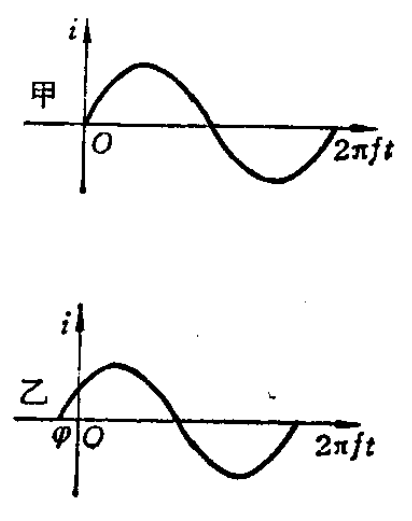
\includegraphics[width=0.8\linewidth]{phase_diagram.png}
    \caption{交流电相位示意图}
    \label{fig:phase_diagram}
\end{figure}

\subsection{相位差}

两个频率相同的交流电相位的差叫做相位差，或者叫做相差。

这两个频率相同的交流电，可以是两个交流电流，可以是两个交流电压，可以是两个交流电动势，也可以是这三种量中的任何两个。例如研究加在电路上的交流电压和通过这个电路的交流电流的相位差。

如果电路是纯电阻，那么交流电压和交流电流的相位差等于零。也就是说交流电压等于零的时候，交流电流也等于零，交流电压变到最大值的时候，交流电流也变到最大值。这种情况叫做同相位，或者叫做同相。

如果电路含有电感和电容，交流电压和交流电流的相位差一般是不等于零的，也就是说一般是不同相的，或者电压超前于电流，或者电流超前于电压。

加在晶体管放大器基极上的交流电压和从集电极输出的交流电压，这两者的相位差正好等于180°。这种情况叫做反相位，或者叫做反相。

\subsection{趋肤效应}

交流电在导体中流过的时候，各处的电流密度不是均匀的。导体内部，电流密度小，越接近导体的表面，电流密度越大。这是由于导体内层比外层有更大的电感，内层感抗大，对交流电的阻碍作用也就大。交流电趋向于从导体表面流过的现象叫做趋肤效应。

交流电的频率越高，趋肤效应越显著。收音机磁性天线上的线圈要用多股线绕制，就是考虑到趋肤效应。用多股线可以增大表面积，高频电流就较容易通过。电视的室外天线一般是用金属管而不用金属棍制作，也是考虑到趋肤效应。对于粗细相同的金属管和金属棍来说，效果基本上是一样的，而金属管要轻得多。天线的金属管粗些比细些好，也和趋肤效应有关。

\section{电压的基本概念}

河水之所以能够流动，是因为有水位差;电荷之所以能够流动，是因为有电位差。电位差也就是电压。电压是形成电流的原因。在电路中，电压常用U表示。

电压的单位是伏(V),也常用毫伏(mV)或者微伏(μV)做单位。1伏=1000毫伏，1毫伏=1000微伏。

电压可以用电压表测量。测量的时候，把电压表并联在电路上，要选择电压表指针接近满偏转的量程。如果电路上的电压大小估计不出来，要先用大的量程，粗略测量后再用合适的量程。这样可以防止由于电压过大而损坏电压表。

\section{电阻的基本概念}

电路中对电流通过有阻碍作用并且造成能量消耗的部分叫做电阻。电阻常用R表示。

电阻的单位是欧(Ω)，也常用千欧(kΩ)或者兆欧(MΩ)做单位。1千欧=1000欧，1兆欧=1000000欧。

导体的电阻由导体的材料、横截面积和长度决定。

电阻可以用万用电表欧姆档测量。测量的时候，要选择电表指针接近偏转一半的欧姆档。如果电阻在电路中，要把电阻的一头烫开后再测量。

\section{欧姆定律}

导体中的电流I和导体两端的电压U成正比，和导体的电阻R成反比，这个规律叫做欧姆定律。即：

\[ I = \frac{U}{R} \]

其中，I为电流，单位是安(A)；U为电压，单位是伏(V)；R为电阻，单位是欧(Ω)。

如果知道电压、电流、电阻三个量中的两个，就可以根据欧姆定律求出第三个量：

\[ U = IR \]
\[ R = \frac{U}{I} \]

在交流电路中，欧姆定律同样成立，但电阻R应该改成阻抗Z，即：

\[ I = \frac{U}{Z} \]

其中，Z为阻抗，单位是欧(Ω)。

\section{阻抗匹配的基本概念}

阻抗匹配是指负载阻抗从设备中获得最大功率的措施。最简单的例子是负载阻抗和电源的内阻抗都是纯电阻的情况。在这种情况中，如果负载电阻小于或者大于电源内电阻，负载电阻获得的功率都是比较小的，只有使负载电阻等于电源内电阻，负载电阻才获得最大的功率。这种使负载电阻等于电源内电阻，从而获得最大功率的措施就叫做匹配。

如果负载阻抗和电源内阻抗不是纯电阻，要做到匹配就复杂一些，不但要求电阻部分相等，而且要求电抗部分大小相等符号相反。电抗包含感抗和容抗，在串联电路中，电抗等于感抗和容抗之差。

在电子电路中，选择负载电阻，使电子器件处于最佳工作状态下输出最大功率，通常也叫做匹配。

在传输线中，使负载阻抗等于传输线的特性阻抗，也叫做匹配。它的目的是消除负载引起的反射，使负载获得最大功率。电视天线的匹配就属于这种情况。

\section{电源的基本概念}

把其他形式的能转换成电能的装置叫做电源。发电机能把机械能转换成电能，干电池能把化学能转换成电能。发电机、干电池等都叫做电源。

通过变压器和整流器，把交流电变成直流电的装置叫做整流电源。

能提供信号的电子设备叫做信号源。晶体三极管能把前面送来的信号加以放大，又把放大了的信号传送到后面的电路中去。晶体三极管对后面的电路来说也可以看作是信号源。

整流电源、信号源有时也叫做电源。

\section{电动势的基本概念}

电动势是反映电源把其他形式的能转换成电能的本领的物理量。电动势使电源两端产生电压。在电路中，电动势常用$\mathcal{E}$表示。电动势的单位和电压的单位相同，也是伏(V)。

电源的电动势可以用电压表测量。测量的时候，电源不要接到电路中去，用电压表测量电源两端的电压，所得的电压值就可以看作等于电源的电动势。如果电源接在电路中，用电压表测得的电源两端的电压就会小于电源的电动势。这是因为电源有内电阻。在闭合的电路中，电流通过内电阻有内电压降，通过外电阻$R$有外电压降。电源的电动势$\mathcal{E}$等于内电压$U_r$和外电压$U_R$之和，即：

\[ \mathcal{E} = U_r + U_R \]

严格来说，即使电源不接入电路，用电压表测量电源两端电压，电压表成了外电路，测得的电压也小于电动势。但是，由于电压表的内电阻很大，电源的内电阻很小，内电压可以忽略。因此，电压表测得的电源两端的电压是可以看作等于电源电动势的。

\begin{figure}[htbp]
    \centering
    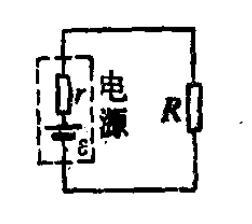
\includegraphics[width=0.8\linewidth]{emf_measurement.png}
    \caption{电源电动势测量示意图}
    \label{fig:emf_measurement}
\end{figure}

\subsubsection{干电池的使用与判断}

干电池用旧了，用电压表测量电池两端的电压，有时候仍然比较高，但是接入电路后却不能使负载(收音机、录音机等)正常工作。这种情况是因为电池的内电阻变大了，甚至比负载的电阻还大，但是仍然比电压表的内电阻小。

用电压表测量电池两端电压的时候，电池内电阻分得的内电压还不大，所以电压表测得的电压仍然比较高。但是电池接入电路后，电池内电阻分得的内电压增大，负载电阻分得的电压就减小，因此不能使负载正常工作。

为了判断旧电池能不能用，应该在有负载的时候测量电池两端的电压。

\subsubsection{稳压电源的性能}

有些性能较差的稳压电源，有负载和没有负载两种情况下测得的电源两端的电压相差较大，也是因为电源的内电阻较大造成的。

\section{负载的基本概念}

把电能转换成其他形式的能的装置叫做负载。电动机能把电能转换成机械能，电阻能把电能转换成热能，电灯泡能把电能转换成热能和光能，扬声器能把电能转换成声能。电动机、电阻、电灯泡、扬声器等都叫做负载。

晶体三极管对于前面的信号源来说，也可以看作是负载。

\section{电路的基本概念}

电流流过的路叫做电路。最简单的电路由电源、负载和导线、开关等元件组成。

电路处处连通叫做通路。只有通路，电路中才有电流通过。

电路某一处断开叫做断路或者开路。

电路某一部分的两端直接接通，使这部分的电压变成零，叫做短路。

\section{LC谐振电路基础}

LC谐振电路是无线电电路的基础，由电感（L）和电容（C）组成，能够选择特定频率的信号。LC谐振电路的工作原理基于电感和电容的谐振特性：当电路的谐振频率与输入信号的频率相同时，电路对该频率的信号呈现最大的阻抗（并联谐振）或最小的阻抗（串联谐振），从而实现频率选择。

\subsection{电感和电容的基本特性}

电感（L）和电容（C）是LC谐振电路的两个基本元件，它们具有不同的电气特性。电感是一种能够储存磁场能量的元件，当电流通过电感时，会在电感周围产生磁场。电感的特性是阻碍电流的变化，电流变化越快，电感产生的感应电压越大。电感的单位是亨利（H），常用单位还有毫亨（$\text{mH}$）和微亨（$\mu\text{H}$）。电感的主要参数包括电感值、直流电阻、品质因数、自谐振频率等。电感的电感值越大，储存的磁场能量越多；直流电阻越小，损耗越小；品质因数越高，损耗越小，选择性越好；自谐振频率越高，工作频率范围越宽。

电容是一种能够储存电场能量的元件，当电压施加在电容两端时，会在电容极板之间产生电场。电容的特性是阻碍电压的变化，电压变化越快，电容产生的电流越大。电容的单位是法拉（F），常用单位还有微法（$\mu\text{F}$）和皮法（$\text{pF}$）。电容的主要参数包括电容值、耐压值、损耗因数、绝缘电阻等。电容的电容值越大，储存的电场能量越多；耐压值越高，能够承受的电压越大；损耗因数越小，损耗越小；绝缘电阻越大，漏电流越小。

\subsection{LC串联谐振电路}

LC串联谐振电路由电感和电容串联连接组成。当感抗等于容抗时，电路发生谐振：

\begin{itemize}[leftmargin=3.5em]
    \item 感抗：$X_L = 2\pi f L$
    \item 容抗：$X_C = \frac{1}{2\pi f C}$
    \item 谐振时：$X_L = X_C$
\end{itemize}

\subsubsection{谐振频率}

谐振频率是LC电路发生谐振时的频率，计算公式为：

\[ f_0 = \frac{1}{2\pi \sqrt{LC}} \]

其中，$f_0$为谐振频率，单位为赫兹（Hz）；L为电感，单位为亨利（H）；C为电容，单位为法拉（F）。

\subsubsection{串联谐振特性}

\begin{itemize}[leftmargin=3.5em]
    \item 阻抗最小：$Z = R$（R为电路中的电阻）
    \item 电流最大：$I = \frac{U}{R}$
    \item 电感和电容两端电压相位相反，大小相等
    \item 电感或电容两端电压可能远大于电源电压（电压谐振）
\end{itemize}

\subsection{LC并联谐振电路}

LC并联谐振电路由电感和电容并联连接组成。谐振条件与串联谐振相同：$X_L = X_C$。

\subsubsection{谐振频率}

并联谐振频率与串联谐振频率相同：

\[ f_0 = \frac{1}{2\pi \sqrt{LC}} \]

\subsubsection{并联谐振特性}

\begin{itemize}[leftmargin=3.5em]
    \item 阻抗最大：$Z = \frac{L}{CR}$
    \item 总电流最小
    \item 电感和电容支路电流相位相反，大小相等
    \item 支路电流可能远大于总电流（电流谐振）
\end{itemize}

\subsection{LC电路的能量转换过程}

LC谐振电路的本质是电感和电容之间的能量转换过程。在谐振状态下，电感和电容之间不断地进行能量交换，形成电磁振荡。当电流通过电感时，电感储存磁场能量，磁场能量为$W_L = \frac{1}{2}LI^2$，其中L是电感值，I是电流。当电压施加在电容两端时，电容储存电场能量，电场能量为$W_C = \frac{1}{2}CV^2$，其中C是电容值，V是电压。

在LC谐振电路中，电感和电容的能量相互转换。当电容放电时，电场能量转换为磁场能量，电流增大，电感储存磁场能量；当电感放电时，磁场能量转换为电场能量，电流减小，电容储存电场能量。这种能量转换过程以谐振频率不断重复，形成持续的电磁振荡。在理想情况下（无损耗），能量转换过程可以无限持续，总能量保持不变。在实际电路中，由于电感和电容存在损耗，能量会逐渐衰减，需要外部能量补充才能维持振荡。

\subsection{品质因数（Q值）}

\subsubsection{Q值的定义}

品质因数是衡量谐振电路性能的重要参数：

\begin{itemize}[leftmargin=3.5em]
    \item 串联电路Q值：$Q = \frac{X_L}{R} = \frac{X_C}{R}$
    \item 并联电路Q值：$Q = \frac{R}{X_L} = \frac{R}{X_C}$
\end{itemize}

\subsubsection{Q值的意义}

\begin{itemize}[leftmargin=3.5em]
    \item Q值越高，谐振曲线越尖锐
    \item 选择性越好，通频带越窄
    \item 能量损耗越小，电路效率越高
\end{itemize}

\subsubsection{提高Q值的方法}

Q值是衡量LC谐振电路性能的重要参数，提高Q值可以显著改善电路的选择性和性能。以下是提高Q值的详细方法：

\begin{enumerate}[leftmargin=3.5em]
    \item \textbf{选择高质量的元件}
    \begin{itemize}
        \item \textbf{电感}：选择低损耗的电感，如空气芯电感或磁芯电感（铁氧体磁芯）
        \item \textbf{电容}：选择低损耗的电容，如聚苯乙烯电容、聚四氟乙烯电容或云母电容
        \item \textbf{电阻}：使用高精度、低温度系数的电阻
    \end{itemize}
    
    \item \textbf{优化电感设计}
    \begin{itemize}
        \item \textbf{减少直流电阻}：使用粗导线绕制电感
        \item \textbf{选择合适的磁芯材料}：高频电路使用高频磁芯
        \item \textbf{优化绕制工艺}：减少匝间电容和损耗
    \end{itemize}
    
    \item \textbf{优化电容选择}
    \begin{itemize}
        \item \textbf{选择低损耗因数（tanδ）的电容}
        \item \textbf{避免使用电解电容}（损耗较大）
        \item \textbf{注意电容的额定电压}：留有足够的电压余量
    \end{itemize}
    
    \item \textbf{减少分布参数的影响}
    \begin{itemize}
        \item \textbf{优化电路布局}：减少引线长度，避免交叉布线
        \item \textbf{使用屏蔽措施}：减少外部干扰
        \item \textbf{合理接地}：减少接地电阻
    \end{itemize}
    
    \item \textbf{减少负载影响}
    \begin{itemize}
        \item \textbf{使用合适的阻抗匹配}：避免负载对Q值的影响
        \item \textbf{采用缓冲电路}：隔离负载与谐振电路
    \end{itemize}
    
    \item \textbf{温度控制}
    \begin{itemize}
        \item \textbf{保持稳定的工作温度}：温度变化会影响元件参数
        \item \textbf{选择温度系数小的元件}：减少温度对Q值的影响
    \end{itemize}
    
    \item \textbf{频率选择}
    \begin{itemize}
        \item \textbf{避开元件的自谐振频率}：防止元件自身谐振影响Q值
        \item \textbf{选择合适的工作频率}：在元件的最佳工作频率范围内
    \end{itemize}
    
    \item \textbf{电路结构优化}
    \begin{itemize}
        \item \textbf{使用抽头式电感}：提高Q值
        \item \textbf{采用并联谐振电路}：在某些情况下Q值更高
        \item \textbf{使用调谐回路}：精细调整谐振频率
    \end{itemize}
\end{enumerate}

\subsubsection{实际应用中的考虑因素}

在实际应用中提高Q值时，需要考虑以下因素：

\begin{itemize}[leftmargin=3.5em]
    \item \textbf{成本与性能平衡}：高质量元件通常成本更高
    \item \textbf{体积与重量限制}：某些高Q值元件体积较大
    \item \textbf{可靠性与稳定性}：确保在各种环境条件下的稳定工作
    \item \textbf{频率范围}：不同频率范围需要不同的元件选择
\end{itemize}

\subsubsection{应用示例：提高收音机调谐回路的Q值}

以收音机调谐回路为例，提高Q值的具体措施包括：

\begin{itemize}[leftmargin=3.5em]
    \item 使用高品质空气芯电感
    \item 选择银云母电容
    \item 优化电路布局，减少引线长度
    \item 采用屏蔽措施，减少外部干扰
    \item 精细调整调谐回路，确保谐振频率准确
\end{itemize}

通过以上方法，可以显著提高LC电路的Q值，从而改善电路的选择性和性能。

\subsection{LC电路的带宽}

\subsubsection{带宽定义}

带宽是电路能够有效工作的频率范围，计算公式为：

\[ BW = \frac{f_0}{Q} \]

\subsubsection{带宽与Q值的关系}

Q值越高，带宽越窄，选择性越好；Q值越低，带宽越宽，选择性越差。

\subsection{阻抗特性曲线和频率响应}

LC谐振电路的阻抗特性随频率变化而变化，形成特定的频率响应曲线。对于串联谐振电路，阻抗随频率的变化呈现V形曲线：在谐振频率处，阻抗最小，等于电路的电阻；在偏离谐振频率时，阻抗逐渐增大。对于并联谐振电路，阻抗随频率的变化呈现倒V形曲线：在谐振频率处，阻抗最大；在偏离谐振频率时，阻抗逐渐减小。

频率响应曲线描述了LC谐振电路对不同频率信号的响应特性。对于串联谐振电路，电流响应曲线与阻抗响应曲线相反：在谐振频率处，电流最大；在偏离谐振频率时，电流逐渐减小。对于并联谐振电路，电压响应曲线与阻抗响应曲线相同：在谐振频率处，电压最大；在偏离谐振频率时，电压逐渐减小。

\subsection{LC电路的应用}

\subsubsection{选频电路}

用于从多个频率信号中选择特定频率，如收音机的调谐电路。

\subsubsection{滤波电路}

滤除不需要的频率成分，如电源滤波、信号滤波等。

\subsubsection{振荡电路}

产生特定频率的正弦波信号，如振荡器、信号源等。

\subsubsection{调谐电路}

收音机、电视机中的频道选择电路。

\subsubsection{匹配电路}

实现阻抗匹配，提高信号传输效率。

\subsubsection{延时电路}

利用LC电路的充放电特性实现信号延时。

\subsection{实际LC电路的考虑因素}

\subsubsection{元件损耗}

实际电感和电容都有损耗，会影响Q值。

\subsubsection{分布参数}

电路布线的分布电感和电容会影响电路性能。

\subsubsection{温度影响}

温度变化会影响元件参数，进而影响谐振频率。

\subsubsection{频率范围}

不同频率范围需选择不同类型的电感和电容。

\subsubsection{稳定性}

需要考虑元件参数的稳定性，如温度系数、老化等。

\section{放大器的基本概念}

能够将微弱信号放大的电子装置叫做放大器。它由电子器件(晶体管或者电子管)、电路元件(电阻、电容等)和电源组成。

放大器的分类方法很多：

\begin{itemize}[leftmargin=3.5em]
    \item \textbf{按工作频率区分}：有直流放大器、低频放大器(音频放大器)、高频放大器(射频放大器)、视频放大器(宽频带放大器)等
    \item \textbf{按用途区分}：有电压放大器(前置放大器、小信号放大器)、功率放大器(大信号放大器)等
    \item \textbf{按工作状态区分}：有甲类放大器、乙类放大器、甲乙类放大器、丙类放大器等
    \item \textbf{按耦合方式区分}：有直接耦合放大器(直流放大器)、阻容耦合放大器、变压器耦合放大器等
\end{itemize}

由于放大器分类的方法很多，同一个放大器可以有几个名称。例如做音频放大的阻容耦合放大器又叫做音频放大器、甲类放大器、电压放大器等。

\subsection{放大器的工作状态}

\subsubsection{甲类放大器}
甲类放大器的特点是在输入信号的整个周期内，晶体管都处于导通状态。这种放大器的优点是输出波形失真小，线性度好，但缺点是效率低，因为晶体管始终有电流通过，即使没有输入信号时也会消耗功率。甲类放大器的效率通常只有25\%左右。

\subsubsection{乙类放大器}
乙类放大器的特点是在输入信号的半个周期内，晶体管处于导通状态，另半个周期则截止。这种放大器的优点是效率高，理论效率可达78.5\%，但缺点是输出波形会产生交越失真，需要采用推挽电路来改善。

\subsubsection{甲乙类放大器}
甲乙类放大器是甲类和乙类的结合，晶体管在输入信号的大部分周期内导通，只有在信号接近零的小范围内截止。这种放大器既保证了较高的效率（通常为50\%-70\%），又减少了交越失真，是音频功率放大器中最常用的工作状态。

\subsubsection{丙类放大器}
丙类放大器的特点是晶体管只在输入信号的小部分周期内导通，效率很高，理论效率可达85\%以上，但输出波形失真较大。丙类放大器主要用于高频功率放大，通过调谐回路来恢复信号波形，广泛应用于无线电发射机中。

\subsection{反馈}

反馈是指从放大器的输出端取出一部分电压或者电流信号，通过一定的电路送回到输入端。反馈可以分为正反馈和负反馈两种。

\begin{itemize}[leftmargin=3.5em]
    \item \textbf{正反馈}：输出信号反馈回到输入端，使放大器的放大倍数增大的反馈。正反馈常常用在再生式收音机中，也可以利用正反馈使放大器产生自激振荡，做成振荡器。
    \item \textbf{负反馈}：输出信号反馈回到输入端，使放大器的放大倍数减小的反馈。负反馈虽然使放大器的放大倍数下降，但是它能够提高放大器的稳定性，改善频率特性，减小波形失真等。因此，负反馈在放大器中使用得十分普遍。
\end{itemize}

负反馈还可分成电压串联负反馈，电流串联负反馈，电压并联负反馈，电流并联负反馈等。

\section{晶体管放大电路基础}

晶体管是无线电电路中最基本的有源器件，具有放大信号和开关控制的功能。在无线电设备中，晶体管放大电路用于放大微弱的射频信号，使其达到足够的功率进行传输或解调。

\subsection{半导体器件基本原理}

半导体器件是利用半导体材料的导电特性制成的电子器件。常用的半导体材料有硅（Si）和锗（Ge），通过掺杂可以形成N型半导体和P型半导体。

\begin{itemize}[leftmargin=3.5em]
    \item \textbf{PN结}：N型半导体与P型半导体结合形成PN结，具有单向导电特性
    \item \textbf{二极管}：由一个PN结构成，用于整流、检波和稳压
    \item \textbf{三极管（BJT）}：由两个PN结构成，分为NPN型和PNP型，具有电流放大功能
    \item \textbf{场效应管（FET）}：利用电场控制电流，分为JFET和MOSFET，输入阻抗高、噪声低
\end{itemize}

在无线电电路中，场效应管（特别是MOSFET）因其高频特性好、噪声系数低而被广泛应用。三极管则因其增益高、成本低，在低频和中频电路中仍被大量使用。

\subsection{基本放大电路}

基本放大电路是无线电电路的核心组成部分，主要有以下三种组态：

\begin{itemize}[leftmargin=3.5em]
    \item \textbf{共射极放大电路}：电压增益和电流增益都较高，是最常用的放大电路组态，但输入输出阻抗不匹配
    \item \textbf{共基极放大电路}：电流增益接近1，但电压增益高，频带宽，适用于高频放大
    \item \textbf{共集电极放大电路}：电压增益接近1，但输入阻抗高、输出阻抗低，常用作阻抗匹配电路
\end{itemize}

放大电路的主要性能指标包括：
\begin{itemize}[leftmargin=3.5em]
    \item \textbf{电压增益}：输出电压与输入电压之比，通常用分贝（dB）表示
    \item \textbf{带宽}：放大电路能够正常工作的频率范围
    \item \textbf{输入/输出阻抗}：影响电路之间的匹配和信号传输效率
    \item \textbf{噪声系数}：衡量放大电路引入噪声大小的指标
    \item \textbf{稳定性}：放大电路在不同条件下保持正常工作的能力
\end{itemize}

\subsection{高频放大电路}

高频放大电路是无线电设备中的关键电路，用于放大射频信号。与低频放大电路相比，高频放大电路需要考虑以下特殊问题：

\begin{itemize}[leftmargin=3.5em]
    \item \textbf{频率响应}：高频放大电路的增益随频率变化，需要在工作频段内保持平坦的频率响应
    \item \textbf{稳定性}：高频下晶体管的内部反馈容易引起自激振荡，需要采取中和或失配等稳定措施
    \item \textbf{阻抗匹配}：高频电路中阻抗匹配至关重要，失配会导致信号反射和功率损失
    \item \textbf{噪声特性}：高频放大电路的噪声系数直接影响接收机的灵敏度
\end{itemize}

常见的高频放大电路类型：
\begin{itemize}[leftmargin=3.5em]
    \item \textbf{调谐放大器}：使用LC谐振回路作为负载，具有选频放大功能，广泛用于收音机的中频放大和射频放大
    \item \textbf{宽带放大器}：使用负反馈或补偿技术实现宽带放大，用于电视和通信设备
    \item \textbf{低噪声放大器（LNA）}：位于接收机前端，要求极低的噪声系数和适当的增益，直接影响接收灵敏度
\end{itemize}

\section{滤波电路}

滤波电路是无线电电路中不可缺少的组成部分，用于选择有用信号、抑制干扰信号。滤波电路按照频率特性可以分为以下几种类型：

\subsection{低通滤波器}

低通滤波器允许低频信号通过，衰减高频信号。在无线电技术中，低通滤波器常用于：

\begin{itemize}[leftmargin=3.5em]
    \item \textbf{电源滤波}：滤除电源中的高频纹波和干扰
    \item \textbf{音频电路}：滤除音频信号中的高频噪声
    \item \textbf{基带信号处理}：在调制和解调过程中限制信号带宽
\end{itemize}

基本的低通滤波器由电阻和电容组成（RC低通滤波器），截止频率为$f_c = \frac{1}{2\pi RC}$。在射频电路中，常用LC低通滤波器，其截止频率为$f_c = \frac{1}{2\pi\sqrt{LC}}$。

\subsection{高通滤波器}

高通滤波器允许高频信号通过，衰减低频信号。在无线电技术中，高通滤波器常用于：

\begin{itemize}[leftmargin=3.5em]
    \item \textbf{耦合电路}：阻隔直流分量，只传输交流信号
    \item \textbf{音频电路}：滤除低频干扰，如电源哼声
    \item \textbf{天线系统}：抑制低频噪声，提高信噪比
\end{itemize}

基本的高通滤波器由电容和电阻组成（CR高通滤波器），截止频率为$f_c = \frac{1}{2\pi RC}$。

\subsection{带通滤波器}

带通滤波器只允许特定频率范围的信号通过，衰减通带以外的信号。在无线电技术中，带通滤波器是最常用的滤波器类型：

\begin{itemize}[leftmargin=3.5em]
    \item \textbf{选频放大}：在接收机中选择特定频率的信号
    \item \textbf{中频放大}：在超外差接收机中提取中频信号
    \item \textbf{频段选择}：在多频段设备中选择工作频段
\end{itemize}

带通滤波器的主要参数包括中心频率$f_0$、带宽BW、品质因数$Q = \frac{f_0}{BW}$等。LC并联谐振回路是最基本的带通滤波器，在无线电电路中广泛应用。

\subsection{带阻滤波器}

带阻滤波器衰减特定频率范围的信号，允许通带以外的信号通过。在无线电技术中，带阻滤波器常用于：

\begin{itemize}[leftmargin=3.5em]
    \item \textbf{干扰抑制}：抑制特定频率的干扰信号
    \item \textbf{镜像频率抑制}：在超外差接收机中抑制镜像频率干扰
    \item \textbf{谐波抑制}：抑制发射机产生的谐波信号
\end{itemize}

常见的带阻滤波器有陷波器（Notch Filter），利用LC串联谐振回路在谐振频率处呈现低阻抗的特性来实现对特定频率的抑制。

\section{混频与振荡电路}

混频与振荡电路是无线电设备中实现频率变换的核心电路，是超外差接收机和发射机不可缺少的组成部分。

\subsection{混频电路原理}

混频电路是将两个不同频率的信号进行非线性组合，产生新的频率分量的过程。混频电路的核心是利用器件的非线性特性实现频率变换。

混频电路的输出信号包含以下频率分量：
\begin{itemize}[leftmargin=3.5em]
    \item \textbf{和频}：$f_1 + f_2$
    \item \textbf{差频}：$|f_1 - f_2|$
    \item \textbf{各次谐波}：$nf_1$、$mf_2$及其组合
\end{itemize}

在超外差接收机中，混频电路将接收到的射频信号（频率为$f_{RF}$）与本机振荡信号（频率为$f_{LO}$）混频，产生中频信号（频率为$f_{IF} = |f_{RF} - f_{LO}|$）。混频电路的主要性能指标包括变频增益、噪声系数、隔离度和线性度等。

\subsection{本机振荡电路}

本机振荡电路产生稳定的射频信号，为混频电路提供本振信号。对振荡电路的基本要求是：

\begin{itemize}[leftmargin=3.5em]
    \item \textbf{频率稳定度}：振荡频率随温度、电源电压等因素的变化要小
    \item \textbf{频谱纯度}：输出信号的相位噪声和杂散要低
    \item \textbf{输出幅度}：输出信号幅度要足够且稳定
    \item \textbf{调谐范围}：能够覆盖所需的工作频率范围
\end{itemize}

常见的振荡电路类型：
\begin{itemize}[leftmargin=3.5em]
    \item \textbf{LC振荡器}：利用LC谐振回路决定振荡频率，如考毕兹振荡器、克拉泼振荡器等
    \item \textbf{晶体振荡器}：利用石英晶体的压电效应产生稳定的振荡信号，频率稳定度极高
    \item \textbf{压控振荡器（VCO）}：通过改变控制电压来调节振荡频率，广泛用于频率合成和锁相环
\end{itemize}

\subsection{频率合成技术}

频率合成技术是利用一个或多个高稳定度的参考频率源，通过加、减、乘、除等运算产生大量离散频率信号的技术。现代无线电设备广泛采用频率合成技术。

\begin{itemize}[leftmargin=3.5em]
    \item \textbf{直接频率合成}：通过混频、分频、倍频等模拟方法直接产生所需频率，频率切换速度快，但电路复杂
    \item \textbf{锁相环频率合成}：利用锁相环（PLL）将VCO的频率锁定在参考频率的整数倍上，具有结构简单、频率稳定度高的优点
    \item \textbf{直接数字频率合成（DDS）}：利用数字技术直接产生频率信号，具有频率分辨率高、切换速度快、可编程等优点
\end{itemize}

锁相环频率合成器是目前应用最广泛的频率合成方案，其基本组成包括参考振荡器、鉴相器、环路滤波器、VCO和可编程分频器。通过改变分频比，可以在很宽的范围内产生大量离散的频率信号。

\section{现代射频集成电路简介}

随着半导体技术的发展，越来越多的无线电电路功能被集成到单个芯片中，形成了射频集成电路（RFIC）。现代无线电设备大量使用射频集成电路，具有体积小、功耗低、可靠性高等优点。

\subsection{射频集成电路发展}

射频集成电路的发展经历了从分立器件到单片集成的过程：

\begin{itemize}[leftmargin=3.5em]
    \item \textbf{分立器件时代}：早期无线电设备使用分立的晶体管、电阻、电容等器件搭建电路
    \item \textbf{模拟集成电路时代}：20世纪70年代开始，将多个功能集成到一块芯片上，如调频/调幅收音机集成电路
    \item \textbf{射频集成电路时代}：20世纪90年代起，随着无线通信的发展，专门的射频集成电路大量出现
    \item \textbf{片上系统（SoC）时代}：将射频前端、基带处理、微处理器等功能全部集成到一块芯片上
\end{itemize}

射频集成电路设计面临的主要挑战包括：高频下的寄生效应、器件模型的准确性、电磁兼容性设计、功耗与性能的平衡等。

\subsection{常用射频芯片}

现代无线电设备中常用的射频芯片包括：

\begin{itemize}[leftmargin=3.5em]
    \item \textbf{低噪声放大器芯片}：如Avago的MGA系列、Mini-Circuits的MMIC系列
    \item \textbf{功率放大器芯片}：如Qorvo、Skyworks的功率放大器模块，广泛用于手机和基站
    \item \textbf{混频器芯片}：如ADI公司的ADL系列混频器，用于频率变换
    \item \textbf{频率合成器芯片}：如TI的LMX系列、ADI的ADF系列锁相环频率合成器
    \item \textbf{收发机芯片}：如Nordic的nRF系列、Espressif的ESP系列无线收发芯片
    \item \textbf{射频开关芯片}：用于天线切换和频段选择，如PE4240等
\end{itemize}

\subsection{软件无线电（SDR）基础}

软件无线电（Software Defined Radio，SDR）是一种将大部分信号处理功能用软件实现的新型无线电技术架构。SDR的核心思想是将模数转换（ADC）和数模转换（DAC）尽可能靠近天线端，用数字信号处理替代传统的模拟电路。

\begin{itemize}[leftmargin=3.5em]
    \item \textbf{基本架构}：天线 $\rightarrow$ 射频前端 $\rightarrow$ ADC/DAC $\rightarrow$ 数字信号处理器（DSP/FPGA）
    \item \textbf{主要优点}：灵活性高，可通过软件升级改变工作模式；多标准兼容，支持多种通信协议
    \item \textbf{关键技术}：高速ADC/DAC、高性能DSP/FPGA、宽带射频前端
    \item \textbf{应用场景}：无线电监测、通信研究、业余无线电、军事通信等
\end{itemize}

常见的SDR平台有：USRP（通用软件无线电外设）、RTL-SDR（基于RTL2832U芯片的低成本SDR）、HackRF One等。SDR技术的发展推动了无线电技术的创新，使得无线电设备的开发更加灵活和高效。

\chapter{信号处理基础}

本章介绍信号处理的基本理论和方法，包括信号分析、傅里叶变换、数字信号处理和现代信号处理技术。信号处理是无线电技术的核心环节。主要内容包括信号的基本概念、系统理论、傅里叶变换与频谱分析、数字信号处理简介和现代信号处理技术。

\section{信号的基本概念}

信号是信息的载体，无线电技术中的信号具有以下基本特性：

\begin{itemize}[leftmargin=3.5em]
    \item \textbf{时域特性}：信号随时间变化的规律
    \item \textbf{频域特性}：信号在频率域的分布特性
    \item \textbf{能量特性}：信号的能量分布和功率特性
    \item \textbf{统计特性}：信号的统计分布规律
\end{itemize}

\subsection{时域特性}

时域分析是研究信号随时间变化的规律，包括信号的幅度、周期、相位等特性。
\begin{itemize}[leftmargin=3.5em]
    \item \textbf{信号的时域表示}：使用时间函数描述信号
    \item \textbf{信号的基本参数}：幅度、周期、频率、相位
    \item \textbf{信号的运算}：加法、乘法、卷积等
\end{itemize}

\subsubsection{频率的历史定义}

从历史角度看，波在一秒钟内所经过的周数叫做频率。用"f"字母表示，频率单位有：周/秒，或称"赫"，简称为周"C"；和千周/秒、兆周/秒，即千周"KC"、兆周"MC"。它们之间换算关系是：

\begin{itemize}[leftmargin=3.5em]
    \item 1MC = 1000KC
    \item 1KC = 1000C
\end{itemize}

这些历史单位在早期无线电技术中被广泛使用，虽然现代标准单位已统一为赫兹（Hz），但了解这些历史单位有助于理解早期无线电技术文献。

\subsection{频域特性}

\subsection{能量与功率特性}

\subsection{声音信号}

声音是一种机械波，是物体振动产生的声波在介质中传播的结果。在无线电技术中，声音通过换能器转换为电信号，再经过处理和传输。

\subsubsection{声音的产生}

声音的产生源于物体的振动。当物体振动时，会引起周围介质（如空气）的振动，形成声波，最终被人耳感知为声音。

通过以下现象可以验证声音由振动产生：
\begin{itemize}[leftmargin=3.5em]
    \item \textbf{锣鼓发声}：用锤击鼓、敲锣时，锣面或鼓面会振动，用手触摸会感到发"麻"；若用手掌按住鼓面停止振动，鼓声会立刻消失
    \item \textbf{人声产生}：说话时用手触摸咽喉，会感觉到咽喉在振动；停止说话时振动停止，声音也随之消失
    \item \textbf{音叉实验}：用小锤打击音叉使其发声，然后将音叉迅速放入水中，水面会溅起水花，证明发声的音叉在振动
\end{itemize}

观察和实验证明：声源总是在振动，只有振动才能发出声音。

\subsubsection{声音的传播}

声音的传播需要介质（媒质）。我们可以通过实验说明声音是通过空气等介质传播的：

在一个玻璃罩里装上电铃，把罩里的空气慢慢地抽掉，使罩里成了真空。在这过程中，可以观察到：当还没有抽气时，通电使电铃发声；随着空气被抽出，电铃声逐渐减弱；当罩内接近真空时，几乎听不见电铃声。这时再把空气从底下放入玻璃罩里，电铃声音又逐渐加强起来。

实验证明，声音不能在真空中传播，只能在空气等媒质中传播。

声音如何通过媒质来传播的呢？当喇叭的纸盆作前后往返运动时，迫使临近的空气随之振动而形成声波，并通过空气的振动把声波自声源向外传播出去。当声波传到人们耳朵里的鼓膜时，鼓膜也就随之振动起来，这时我们就听到了声音。

\begin{figure}[htbp]
    \centering
    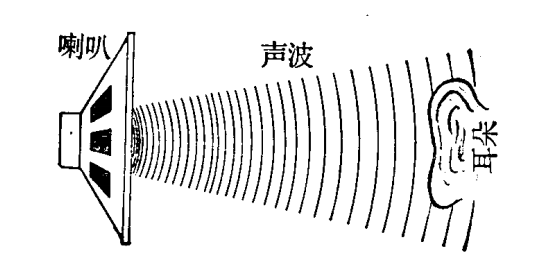
\includegraphics[width=0.8\linewidth]{sound_propagation.png}
    \caption{扬声器发出的声音被耳朵听到的过程}
    \label{fig:sound_propagation}
\end{figure}

声音不仅可以通过空气传播，还可以通过其他介质传播。例如，当潜入水中时，若岸上的人在附近投一块石头，耳朵就会接收到石块落水的声音。这是因为当石块投进水中时，水面会激起水波，水波以石块落水处为中心逐渐向外传播。由于石头落水处的水先产生振动，随后带动周围的水也产生振动，进而在广泛的水域内引起振动。振动就这样一步步地通过水（媒介）向四周传播，而形成水波。

\begin{figure}[htbp]
    \centering
    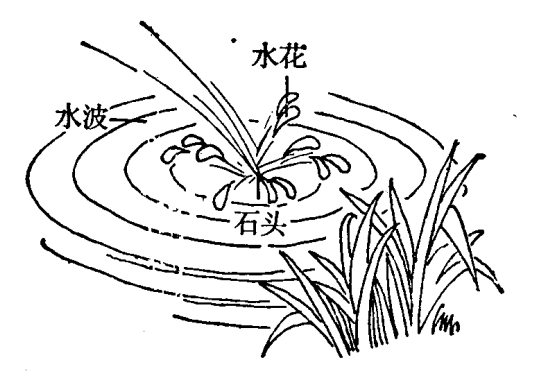
\includegraphics[width=0.6\linewidth]{water_wave.png}
    \caption{石块落水形成的水波传播示意图}
    \label{fig:water_wave}
\end{figure}

\subsubsection{声音信号的传输}

声音在空气中的传播速度很慢，每秒340米，要把声音传到很远地方是不可能的。然而人们的社会活动需要及时听到远方的声音，怎么办？人们就动脑筋想办法使声音变成电的信号，就可以在瞬时间把声音传到很远很远的地方。因为电流的速度特别快，每秒钟是30万公里。

例如电话，就是把声音转变成每秒几十赫到一万赫频率的音频信号电流，然后通过电话线送到很远很远的地方，再由受话器还原成声音。人的耳朵大约只能听到16赫到20000赫范围内的声音（频率），这就叫做"音频"或"低频"。

有线广播就是利用电流传播声音信号的，但输送电流需要铺设大量的导线，有时在铺设过程中会遇到大江湖海或高山，在铺设上困难就很大，并且要花费许多劳力和经费，很不经济。随着科学的发展，人们用无线电波传送声音就很方便。前面说过无线电波的速度与电流的速度一样，每秒钟跑30万公里，它的特点是不要铺设导线，可以向空间四面八方传播，称为无线广播。

现在的问题就是如何想办法让声音"坐"上无线电波飞到世界每一个角落，甚至宇宙深处。

\section{系统的基本概念}

无线电系统是处理信号的装置，具有以下基本特性：

\begin{itemize}[leftmargin=3.5em]
    \item \textbf{线性系统}：满足叠加原理的系统
    \item \textbf{时不变系统}：系统特性不随时间变化的系统
    \item \textbf{因果系统}：输出只依赖于当前和过去输入的系统
    \item \textbf{稳定系统}：有界输入产生有界输出的系统
\end{itemize}

\section{信号与系统的数学描述}

信号与系统的数学描述是无线电技术的基础：

\begin{itemize}[leftmargin=3.5em]
    \item \textbf{傅里叶变换}：时域与频域之间的变换关系
    \item \textbf{拉普拉斯变换}：分析线性时不变系统的工具
    \item \textbf{Z变换}：离散时间系统的分析工具
    \item \textbf{卷积运算}：描述线性系统输入输出关系
\end{itemize}

\section{傅里叶变换与频谱分析}

傅里叶变换是信号处理中最基本的数学工具之一，它将信号从时域转换到频域，揭示信号的频率组成。在无线电技术中，傅里叶变换是分析信号频谱特性、设计滤波器和调制解调电路的理论基础。

\subsection{傅里叶级数}

傅里叶级数适用于周期信号的分析。任何一个满足狄利克雷条件的周期信号，都可以展开为一系列正弦和余弦函数的叠加：

$$f(t) = \frac{a_0}{2} + \sum_{n=1}^{\infty}\left(a_n\cos(n\omega_0 t) + b_n\sin(n\omega_0 t)\right)$$

其中，$\omega_0 = \frac{2\pi}{T}$为基波角频率，$T$为信号周期，$a_n$和$b_n$为傅里叶系数。

\begin{itemize}[leftmargin=3.5em]
    \item \textbf{基波}：频率与原信号频率相同的正弦分量
    \item \textbf{谐波}：频率为基波频率整数倍的正弦分量
    \item \textbf{频谱}：各频率分量的幅度和相位随频率变化的图形
\end{itemize}

在无线电技术中，傅里叶级数常用于分析周期性信号（如方波、锯齿波等）的频谱特性，以及理解调制信号中载波和边带的关系。

\subsection{傅里叶变换}

傅里叶变换将傅里叶级数的概念推广到非周期信号，建立了时域和频域之间的对应关系：

$$F(\omega) = \int_{-\infty}^{+\infty} f(t)e^{-j\omega t}dt$$

傅里叶逆变换为：

$$f(t) = \frac{1}{2\pi}\int_{-\infty}^{+\infty} F(\omega)e^{j\omega t}d\omega$$

\begin{itemize}[leftmargin=3.5em]
    \item \textbf{幅度谱}：$|F(\omega)|$表示信号在各频率上的幅度分布
    \item \textbf{相位谱}：$\arg(F(\omega))$表示信号在各频率上的相位分布
    \item \textbf{能量谱密度}：$|F(\omega)|^2$表示信号能量在各频率上的分布
\end{itemize}

傅里叶变换的重要性质包括线性性、时移性、频移性、尺度变换性、卷积定理等。其中，卷积定理在无线电技术中尤为重要：时域的卷积对应频域的乘积，时域的乘积对应频域的卷积。

\subsection{频谱分析应用}

频谱分析在无线电技术中有广泛的应用：

\begin{itemize}[leftmargin=3.5em]
    \item \textbf{信号分析}：通过频谱分析了解信号的频率组成，判断信号质量
    \item \textbf{调制分析}：分析调幅波、调频波的频谱特性，理解调制过程
    \item \textbf{干扰分析}：通过频谱分析定位干扰信号的频率和强度
    \item \textbf{信道特性分析}：分析信道的频率响应，设计补偿滤波器
    \item \textbf{电磁兼容测试}：测量设备发射的频谱，确保符合标准要求
\end{itemize}

在实际应用中，频谱分析仪是最常用的频谱分析工具，可以直观地显示信号的频谱特性。

\section{数字信号处理简介}

数字信号处理（DSP）是利用数字方法对信号进行处理的技术。与模拟信号处理相比，数字信号处理具有精度高、灵活性强、可重复性好等优点。

\subsection{采样定理}

采样定理（奈奎斯特定理）是数字信号处理的理论基础，它规定了将模拟信号转换为数字信号时采样频率的最低要求：

采样频率$f_s$必须大于信号最高频率$f_{max}$的两倍，即$f_s > 2f_{max}$。

\begin{itemize}[leftmargin=3.5em]
    \item \textbf{奈奎斯特频率}：$f_N = f_s/2$，是采样频率的一半，也是能够正确表示的最高信号频率
    \item \textbf{混叠现象}：当采样频率不满足采样定理时，高频分量会折叠到低频段，造成信号失真
    \item \textbf{抗混叠滤波}：在采样之前使用低通滤波器滤除高于奈奎斯特频率的信号分量
\end{itemize}

在无线电技术中，软件无线电（SDR）系统需要根据工作频段选择合适的采样率和ADC分辨率，以满足系统性能要求。

\subsection{离散傅里叶变换（DFT）}

离散傅里叶变换（DFT）是将离散时间信号转换到离散频率域的数学工具：

$$X(k) = \sum_{n=0}^{N-1}x(n)e^{-j\frac{2\pi}{N}kn}, \quad k = 0, 1, \ldots, N-1$$

\begin{itemize}[leftmargin=3.5em]
    \item \textbf{频率分辨率}：$\Delta f = f_s/N$，采样频率一定时，增加采样点数N可以提高频率分辨率
    \item \textbf{计算量}：直接计算DFT需要$N^2$次复数乘法运算
    \item \textbf{快速傅里叶变换（FFT）}：利用对称性和周期性将计算量降低到$N\log_2 N$次，是DFT的高效算法
\end{itemize}

FFT是数字信号处理中最重要的算法之一，广泛应用于频谱分析、滤波、调制解调等无线电信号处理环节。

\subsection{数字滤波器}

数字滤波器是对数字信号进行频率选择的算法或器件，分为两大类：

\begin{itemize}[leftmargin=3.5em]
    \item \textbf{FIR滤波器}（有限脉冲响应滤波器）：输出只依赖于当前和过去的输入，具有线性相位特性，稳定性好，但阶数较高时计算量大
    \item \textbf{IIR滤波器}（无限脉冲响应滤波器）：输出依赖于当前和过去的输入及输出，可以用较低的阶数实现陡峭的滤波特性，但相位非线性，可能不稳定
\end{itemize}

数字滤波器的设计方法包括窗函数法、频率采样法、双线性变换法等。在无线电设备中，数字滤波器常用于基带信号处理、信道选择和噪声抑制等。

\section{现代信号处理技术}

随着集成电路技术的发展，信号处理技术不断进步，出现了许多新的技术和方法。

\subsection{DSP处理器应用}

数字信号处理器（DSP）是专门为信号处理运算优化的微处理器，具有以下特点：

\begin{itemize}[leftmargin=3.5em]
    \item \textbf{硬件乘加器}：在单个时钟周期内完成乘法和加法运算
    \item \textbf{哈佛架构}：程序存储器和数据存储器分开，可以同时访问指令和数据
    \item \textbf{循环寻址}：硬件支持循环缓冲区操作，适合滤波器等算法
    \item \textbf{饱和运算}：防止溢出造成的信号失真
\end{itemize}

常见的DSP处理器系列有TI的TMS320C6000系列、ADI的SHARC系列等。DSP处理器广泛应用于软件无线电、音频处理、雷达信号处理等领域。

\subsection{FPGA在无线电中的应用}

现场可编程门阵列（FPGA）是一种可编程的逻辑器件，具有并行处理能力强、灵活性高、开发周期短等优点。在无线电技术中，FPGA的应用越来越广泛：

\begin{itemize}[leftmargin=3.5em]
    \item \textbf{数字下变频（DDC）}：将射频信号数字化后，通过FPGA实现数字混频和滤波
    \item \textbf{调制解调}：利用FPGA的高速并行处理能力实现各种调制解调算法
    \item \textbf{协议处理}：实现通信协议的编解码和数据处理
    \item \textbf{实时信号处理}：利用FPGA的并行性实现高速实时信号处理
\end{itemize}

FPGA在5G基站、雷达系统、电子对抗等高性能无线电系统中发挥着重要作用。

\subsection{自适应信号处理}

自适应信号处理是能够根据输入信号和环境的统计特性自动调整参数的信号处理技术。

\begin{itemize}[leftmargin=3.5em]
    \item \textbf{自适应滤波}：滤波器系数根据误差信号自动调整，用于噪声消除、回波抵消和信道均衡
    \item \textbf{自适应天线}：通过调整天线阵列的加权系数，实现波束成形和干扰抑制
    \item \textbf{自适应调制}：根据信道条件自动选择调制方式和编码速率，优化传输效率
\end{itemize}

自适应信号处理在移动通信、雷达、声纳等领域有重要应用，是现代无线电技术的重要组成部分。

\chapter{频谱管理与法规}

本章介绍频谱管理的国际体系、中国频谱管理政策和频谱共享新技术。频谱管理是确保无线电系统有序运行的关键。主要内容包括国际频谱管理体系、中国频谱管理、频谱共享与新技术。

\section{国际频谱管理体系}

\subsection{ITU组织与职能}

\subsection{ITU区域划分}
国际电信联盟将全球划分为三个区域：
\begin{itemize}[leftmargin=3.5em]
    \item \textbf{区域1}：欧洲、非洲、中东和部分亚洲地区
    \item \textbf{区域2}：美洲地区
    \item \textbf{区域3}：亚洲和大洋洲地区
\end{itemize}

\subsection{国际频率分配表}

国际电信联盟（ITU）负责全球无线电频率的分配和管理，确保无线电频谱的有效利用。

\subsubsection{业余无线电频段}
\begin{itemize}[leftmargin=3.5em]
    \item 1.8--2.0MHz：160米波段
    \item 3.5--4.0MHz：80米波段
    \item 7.0--7.3MHz：40米波段
    \item 14.0--14.35MHz：20米波段
    \item 144--146MHz：2米波段
    \item 430--440MHz：70厘米波段
\end{itemize}

\subsubsection{广播频段}
\begin{itemize}[leftmargin=3.5em]
    \item 525--1605kHz：中波广播（AM）
    \item 87--108MHz：调频广播（FM）
    \item 174--230MHz：电视广播VHF频段
    \item 470--862MHz：电视广播UHF频段
\end{itemize}

\subsubsection{移动通信频段}
\begin{itemize}[leftmargin=3.5em]
    \item 800MHz：2G/3G/4G通信
    \item 900MHz：GSM通信
    \item 1800MHz：DCS通信
    \item 2.1GHz：3G通信
    \item 2.6GHz：4G通信
    \item 3.5GHz：5G通信
    \item 24GHz：5G毫米波通信
\end{itemize}

\subsubsection{ISM频段}
\begin{itemize}[leftmargin=3.5em]
    \item 13.56MHz：RFID应用
    \item 2.4GHz：Wi-Fi、蓝牙、微波炉
    \item 5.8GHz：Wi-Fi、雷达
    \item 60GHz：高速无线通信
\end{itemize}

\section{中国频谱管理}

\subsection{管理体制与法规}

\subsection{主要业务频段划分}

\subsection{台站管理与审批}
无线电台站的管理和规范是确保无线电频谱有序使用的重要保障。
\begin{itemize}[leftmargin=3.5em]
    \item \textbf{台站设置}：无线电台站的设置规范和审批流程
    \item \textbf{使用管理}：台站的日常使用和维护要求
    \item \textbf{频率管理}：台站频率的分配和使用管理
    \item \textbf{监督检查}：台站运行的监督和检查机制
    \item \textbf{干扰处理}：无线电干扰的检测和处理方法
\end{itemize}

\section{频谱共享与新技术}

随着无线通信业务的快速增长，频谱资源日益紧张。频谱共享和新技术成为提高频谱利用效率的重要途径。

\subsection{认知无线电}

认知无线电（Cognitive Radio，CR）是一种能够感知周围电磁环境并智能调整工作参数的无线电技术。认知无线电的核心思想是让无线电设备具备"认知"能力，能够自动检测空闲频谱并利用其进行通信。

\begin{itemize}[leftmargin=3.5em]
    \item \textbf{频谱感知}：实时检测周围频谱的使用状况，识别空闲频段
    \item \textbf{频谱决策}：根据感知结果和业务需求，选择最佳的工作频段和通信参数
    \item \textbf{频谱共享}：在不干扰授权用户的前提下，共享使用空闲频谱
    \item \textbf{频谱迁移}：当检测到授权用户出现时，自动切换到其他空闲频段
\end{itemize}

认知无线电的频谱感知技术包括匹配滤波检测、能量检测、循环平稳特征检测等。其中，能量检测实现简单但精度较低，循环平稳特征检测精度高但计算复杂。

\subsection{动态频谱接入}

动态频谱接入（Dynamic Spectrum Access，DSA）是允许无线电设备根据实时频谱状况动态选择工作频率的技术。与传统的固定频谱分配方式不同，动态频谱接入能够更灵活、高效地利用频谱资源。

\begin{itemize}[leftmargin=3.5em]
    \item \textbf{动态专用模型}：频谱分配给特定用户，但可以根据需求动态调整
    \item \textbf{开放共享模型}：多个用户在不受限制的情况下共享频谱，通过协议避免冲突
    \item \textbf{分层接入模型}：区分主用户和次级用户，次级用户在不干扰主用户的前提下使用频谱
\end{itemize}

动态频谱接入在军事通信、应急通信和物联网等领域有重要应用价值。IEEE 802.22标准就是基于认知无线电技术的无线区域网标准，利用电视广播频段的空闲信道进行宽带无线接入。

\subsection{频谱拍卖机制}

频谱拍卖是各国电信监管机构分配商用频谱资源的主要方式。通过市场化的拍卖机制，将频谱使用权分配给能够最高效利用该资源的运营商。

\begin{itemize}[leftmargin=3.5em]
    \item \textbf{同时多轮拍卖（SMRA）}：多轮竞价，每轮投标人可以同时竞拍多个频谱块
    \item \textbf{组合时钟拍卖（CCA）}：允许投标人对频谱组合进行整体竞价，避免互补性频谱块被分散
    \item \textbf{激励拍卖}：将广播电视频谱从广播电视机构转移到移动通信运营商
\end{itemize}

频谱拍卖的收入通常用于国家财政预算，部分国家将拍卖收入用于推动农村地区通信基础设施建设。近年来，5G频谱拍卖在全球范围内展开，中低频段（如700MHz、3.5GHz）和毫米波频段（如26GHz、40GHz）成为拍卖热点。

\chapter{无线电测量与测试技术}

\section{测量基础理论}

无线电测量的基本原理和技术方法：

\subsection{频谱分析技术}

\begin{itemize}[leftmargin=3.5em]
    \item \textbf{分辨率带宽（RBW）}：影响频谱分辨能力的关键参数
    \item \textbf{视频带宽（VBW）}：影响显示平滑度和测量精度
    \item \textbf{扫描时间}：影响测量精度和实时性
    \item \textbf{参考电平}：设置合适的显示范围和测量范围
\end{itemize}

\subsection{网络分析技术}

\begin{itemize}[leftmargin=3.5em]
    \item \textbf{S参数测量}：S11、S21等参数的意义和应用
    \item \textbf{阻抗测量}：天线输入阻抗的精确测量方法
    \item \textbf{驻波比测量}：评估天线匹配状态的重要指标
    \item \textbf{相位测量}：信号相位的精确测量技术
\end{itemize}

\subsection{功率测量技术}

\begin{itemize}[leftmargin=3.5em]
    \item \textbf{平均功率}：信号的平均功率水平测量
    \item \textbf{峰值功率}：信号的瞬时最大功率测量
    \item \textbf{脉冲功率}：脉冲信号的功率特性分析
    \item \textbf{功率校准}：确保测量精度的校准方法
\end{itemize}

\subsection{调制质量评估}

\begin{itemize}[leftmargin=3.5em]
    \item \textbf{调制深度}：AM调制的深度测量和分析
    \item \textbf{频偏测量}：FM调制的频偏大小测量
    \item \textbf{调制失真}：调制过程中的失真程度评估
    \item \textbf{误码率}：数字调制的质量指标测量
\end{itemize}

\section{测试仪器介绍}

常用无线电测试仪器的工作原理和使用方法：

\subsection{频谱分析仪}

\begin{itemize}[leftmargin=3.5em]
    \item \textbf{工作原理}：基于超外差接收机原理
    \item \textbf{主要功能}：频谱显示、功率测量、调制分析
    \item \textbf{关键技术}：频率合成、数字信号处理
    \item \textbf{应用场景}：信号监测、干扰分析、设备测试
\end{itemize}

\subsection{信号发生器}

\begin{itemize}[leftmargin=3.5em]
    \item \textbf{工作原理}：直接数字合成（DDS）技术
    \item \textbf{主要功能}：信号产生、调制、扫描
    \item \textbf{关键技术}：频率精度、相位噪声、调制质量
    \item \textbf{应用场景}：设备测试、系统校准、教学实验
\end{itemize}

\subsection{网络分析仪}

\begin{itemize}[leftmargin=3.5em]
    \item \textbf{工作原理}：矢量网络分析技术
    \item \textbf{主要功能}：S参数测量、阻抗分析、时域分析
    \item \textbf{关键技术}：误差校正、时域门控
    \item \textbf{应用场景}：天线测试、滤波器设计、电缆测试
\end{itemize}

\subsection{功率计}

\begin{itemize}[leftmargin=3.5em]
    \item \textbf{工作原理}：热电偶或二极管检测
    \item \textbf{主要功能}：功率测量、功率校准
    \item \textbf{关键技术}：传感器线性度、频率响应
    \item \textbf{应用场景}：发射机功率测量、系统功率监测
\end{itemize}

\section{电磁兼容测试}

电磁兼容测试的基本原理和技术要求：

\subsection{屏蔽技术原理}

\begin{itemize}[leftmargin=3.5em]
    \item \textbf{电场屏蔽}：使用导电材料屏蔽电场干扰
    \item \textbf{磁场屏蔽}：使用高导磁材料屏蔽磁场干扰
    \item \textbf{电磁屏蔽}：综合屏蔽电磁场干扰
    \item \textbf{屏蔽效能}：衡量屏蔽效果的重要指标
\end{itemize}

\subsection{滤波技术应用}

\begin{itemize}[leftmargin=3.5em]
    \item \textbf{低通滤波}：滤除高频干扰，保留低频信号
    \item \textbf{高通滤波}：滤除低频干扰，保留高频信号
    \item \textbf{带通滤波}：选择特定频段信号传输
    \item \textbf{带阻滤波}：抑制特定频段干扰信号
\end{itemize}

\subsection{接地技术要点}

\begin{itemize}[leftmargin=3.5em]
    \item \textbf{单点接地}：减少地环路干扰的有效方法
    \item \textbf{多点接地}：降低接地阻抗，提高接地效果
    \item \textbf{混合接地}：结合单点和多点接地的优化方案
    \item \textbf{接地电阻}：衡量接地效果的关键参数
\end{itemize}

\subsection{布线技术规范}

\begin{itemize}[leftmargin=3.5em]
    \item \textbf{信号线分离}：强弱信号线分开布线，减少干扰
    \item \textbf{电源线滤波}：电源线加装滤波器，抑制电源干扰
    \item \textbf{屏蔽线使用}：敏感信号使用屏蔽线，提高抗干扰能力
    \item \textbf{布线长度控制}：控制布线长度，减少信号衰减和干扰
\end{itemize}

\section{安全测试要求}

无线电设备的安全测试标准和要求：

\subsection{辐射发射测试}

\begin{itemize}[leftmargin=3.5em]
    \item \textbf{测试标准}：CISPR、FCC等国际标准要求
    \item \textbf{测试环境}：电波暗室或开阔场测试环境
    \item \textbf{测试距离}：3米、10米等不同测试距离
    \item \textbf{限值要求}：不同频段的发射限值标准
\end{itemize}

\subsection{抗扰度测试}

\begin{itemize}[leftmargin=3.5em]
    \item \textbf{静电放电}：模拟人体静电放电的抗扰度测试
    \item \textbf{射频场抗扰度}：模拟外部射频干扰的抗扰度测试
    \item \textbf{电快速瞬变}：模拟开关瞬态干扰的抗扰度测试
    \item \textbf{浪涌抗扰度}：模拟雷击等大电流冲击的抗扰度测试
\end{itemize}

\subsection{谐波测试}

\begin{itemize}[leftmargin=3.5em]
    \item \textbf{谐波电流}：设备产生的谐波电流测量
    \item \textbf{测量方法}：使用功率分析仪进行精确测量
    \item \textbf{限值要求}：不同功率等级的谐波限值标准
    \item \textbf{抑制措施}：功率因数校正等谐波抑制技术
\end{itemize}

\subsection{静电放电测试}

\begin{itemize}[leftmargin=3.5em]
    \item \textbf{测试等级}：接触放电和空气放电的不同等级
    \item \textbf{测试点}：设备外壳、接口等关键测试位置
    \item \textbf{测试方法}：标准化的静电放电测试流程
    \item \textbf{防护措施}：静电防护设计和材料选择
\end{itemize}

\part{无线电技术应用与发展}

\chapter{技术发展历程}

本章回顾无线电技术从诞生到现代的重要发展历程，包括早期发展阶段、技术突破阶段、数字化阶段和现代发展阶段。了解技术发展历程有助于理解无线电技术的演进规律。

无线电技术从诞生到现代的重要发展历程：

\section{早期发展阶段（1895-1940）}

无线电技术的早期发展奠定了现代通信的基础：

\begin{itemize}[leftmargin=3.5em]
    \item \textbf{1895年}：马可尼实现首次无线电通信，距离约3公里
    \item \textbf{1906年}：费森登进行首次无线电广播，播放音乐和讲话
    \item \textbf{1912年}：泰坦尼克号事件推动海上无线电通信发展
    \item \textbf{1920年代}：商业广播电台开始运营
\end{itemize}

\section{技术突破阶段（1940-1980）}

这一阶段见证了无线电技术的重大突破：

\begin{itemize}[leftmargin=3.5em]
    \item \textbf{1947年}：贝尔实验室发明晶体管，开启固态电子时代
    \item \textbf{1950年代}：电视广播开始普及
    \item \textbf{1960年代}：卫星通信技术发展
    \item \textbf{1970年代}：集成电路技术成熟，设备小型化
\end{itemize}

\section{数字化阶段（1980-2000）}

数字化技术推动了无线电技术的革命性发展：

\begin{itemize}[leftmargin=3.5em]
    \item \textbf{1980年代}：移动电话开始商用
    \item \textbf{1990年代}：数字信号处理技术广泛应用
    \item \textbf{1990年代}：GSM数字移动通信标准制定
    \item \textbf{1990年代}：互联网与无线技术开始融合
\end{itemize}

\section{现代发展阶段（2000至今）}

现代无线电技术呈现出多元化、智能化的发展趋势：

\begin{itemize}[leftmargin=3.5em]
    \item \textbf{2000年代}：3G移动通信商用，软件定义无线电技术发展
    \item \textbf{2010年代}：4G LTE技术普及，认知无线电技术应用
    \item \textbf{2020年代}：5G技术大规模部署，毫米波通信商用
    \item \textbf{2020年代后期}：6G技术研究启动，太赫兹通信、卫星互联网、人工智能与无线电融合
    \item \textbf{2025年代展望}：空天地一体化网络，量子通信技术突破，绿色节能通信技术
\end{itemize}

\subsection{2020年代技术突破}

2020年代见证了无线电技术的重大突破：

\begin{itemize}[leftmargin=3.5em]
    \item \textbf{5G-Advanced技术}：增强型5G技术，支持更高精度定位和更低时延
    \item \textbf{毫米波通信}：24-100GHz频段商用，实现太比特级传输速率
    \item \textbf{卫星互联网}：低轨卫星星座（Starlink、OneWeb等）提供全球覆盖
    \item \textbf{人工智能融合}：AI技术在频谱管理、信号处理、网络优化中的应用
    \item \textbf{绿色通信}：能效提升技术，减少无线电设备能耗
\end{itemize}

\subsection{实际应用案例}

2020年代无线电技术的实际应用案例展示了技术创新的价值：

\begin{itemize}[leftmargin=3.5em]
    \item \textbf{5G-Advanced工业应用}：在智能制造中实现超低时延控制，支持工业机器人精准协作
    \item \textbf{毫米波车联网}：利用24GHz频段实现车辆间厘米级定位，支持自动驾驶技术
    \item \textbf{卫星互联网应用}：Starlink为偏远地区提供高速互联网接入，OneWeb为航空、海事提供全球连接
    \item \textbf{AI辅助频谱管理}：利用机器学习算法实现动态频谱分配，提高频谱利用效率
    \item \textbf{绿色通信实践}：运营商通过智能休眠技术，减少基站能耗30%以上
\end{itemize}

\subsection{6G技术发展趋势}

6G技术预计在2030年左右商用，主要发展方向包括：

\begin{itemize}[leftmargin=3.5em]
    \item \textbf{太赫兹通信}：100GHz-10THz频段，支持超高容量通信
    \item \textbf{智能超表面}：可编程电磁表面，实现智能无线环境
    \item \textbf{通感一体化}：通信与感知功能融合，支持环境感知应用
    \item \textbf{量子通信}：基于量子原理的新型安全通信技术
    \item \textbf{空天地一体化}：地面、卫星、空中平台协同组网
\end{itemize}

\chapter{主要应用领域}

本章介绍无线电技术在各个领域的广泛应用，包括通信技术、广播与导航、雷达与遥感和科学研究等。了解应用领域有助于理解无线电技术的实际价值。

\section{通信技术应用}

无线电技术在通信领域的广泛应用体现了基础理论的实际价值：

\subsection{移动通信技术}

移动通信技术的发展展示了无线电技术的演进：

\begin{itemize}[leftmargin=3.5em]
    \item \textbf{5G通信}：3.5GHz、2.6GHz频段，大规模MIMO技术，超高速率低时延
    \item \textbf{4G通信}：LTE技术，2.1GHz、2.6GHz频段，移动宽带服务
    \item \textbf{3G通信}：WCDMA技术，2.1GHz频段，多媒体通信
    \item \textbf{2G通信}：GSM技术，900MHz、1800MHz频段，语音通信
\end{itemize}

\subsection{物联网通信}

物联网通信技术体现了无线电技术在智能化应用中的重要作用：

\begin{itemize}[leftmargin=3.5em]
    \item \textbf{NB-IoT}：900MHz频段，低功耗广域覆盖，智能抄表应用
    \item \textbf{LoRa}：433MHz、868MHz频段，长距离低功耗，农业监测
    \item \textbf{Zigbee}：2.4GHz频段，短距离自组网，智能家居
    \item \textbf{Sigfox}：868MHz频段，超低功耗，资产追踪
\end{itemize}

\subsection{卫星通信系统}

卫星通信系统展示了无线电技术在空间通信中的应用：

\begin{itemize}[leftmargin=3.5em]
    \item \textbf{低轨道卫星}：Starlink、OneWeb系统，Ka/Ku频段，全球宽带
    \item \textbf{中轨道卫星}：GPS、北斗系统，L频段，导航定位
    \item \textbf{高轨道卫星}：同步轨道卫星，C/Ku频段，广播电视
    \item \textbf{移动卫星}：天通系统，S频段，应急通信
\end{itemize}

\subsection{车联网技术}

车联网技术体现了无线电技术在智能交通中的应用：

\begin{itemize}[leftmargin=3.5em]
    \item \textbf{C-V2X}：5.9GHz频段，车与车、车与路侧设备通信
    \item \textbf{DSRC}：5.9GHz频段，专用短程通信技术
    \item \textbf{车载雷达}：24GHz、77GHz频段，自动驾驶感知
    \item \textbf{车载通信}：4G/5G模块，远程监控和娱乐服务
\end{itemize}

\section{广播与导航应用}

无线电技术在广播和导航领域的重要应用：

\subsection{广播频段与接收设备}

无线电接收设备主要使用的是中频（MF）、高频（HF）和甚高频（VHF）频段。中频用于AM广播，高频用于短波广播，甚高频用于FM广播。不同频段的无线电波具有不同的传播特性，需要使用不同类型的天线和接收电路。

具体来说，收音机一般使用以下波段：
\begin{itemize}[leftmargin=3.5em]
    \item \textbf{中波}：频率范围为535kHz-1605kHz
    \item \textbf{短波}：频率范围为2000kHz-24000kHz，常用3500kHz-18000kHz
\end{itemize}

有的收音机将短波分为短波1、短波2等多个波段，以方便接收不同频率范围的信号。

\subsection{无线电广播的发射与接收}

\subsubsection{广播发射过程}

在无线电广播电台里，都装有高频振荡器。高频振荡器会产生一种用来运载声音信号的无线电波，我们称它为"载波"，它具有一定的幅度和频率。有了载波，声音还不能直接"坐"上载波，必须先用微音器，如"话筒"把语言、音乐等声音信号转变成强度随声音信号而变化的音频电流，由于这个音频电流很微弱，要把这微弱的音频电流通过音频放大器进行放大，再把放大的音频电流叠加到高频电流上（即高频载波信号电流），这个过程叫"调制"。

调制方法有两种：一种是"调幅"制，另一种是"调频"制，经过调制，高频载波信号就把低频信号载上了（好比飞机把乘客载上了一样）。接着就是研究如何让载波"起飞"的问题了。

从"调制器"输出的调幅波送入放大器使调制的载波电流信号放大，以增强能量，然后通过天线向空中发射出去（好比飞机载着乘客飞往世界各地一样），这就是无线电波发射的一般过程。

\begin{figure}[htbp]
    \centering
    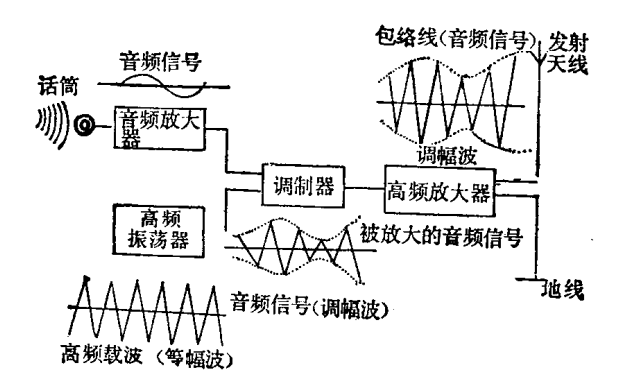
\includegraphics[width=0.8\linewidth]{radio_transmission.png}
    \caption{无线电波发射过程示意图}
    \label{fig:radio_transmission}
\end{figure}

\subsubsection{调幅与调频}

我国各省市广播电台普遍采用的是"调幅"制，"调幅"制产生的无线电波就叫调幅波，采用调幅方式的广播叫做调幅广播。什么叫"调幅"呢？调幅是把等幅高频振荡电流，变成振幅随音频信号而变化的高频振荡电流。

采用调频波的广播方式叫调频广播。什么叫做调频呢？就是高频电流的频率随着音频信号的变化而变化。

调幅和调频的特点不一样。一般中波和短波都是应用调幅广播。例如，中央人民广播电台和各地人民广播电台。而调频广播用超短波，例如电视广播中的伴音部分等。

\subsubsection{广播接收过程}

无线电波又是如何被接收的呢？

\begin{figure}[htbp]
    \centering
    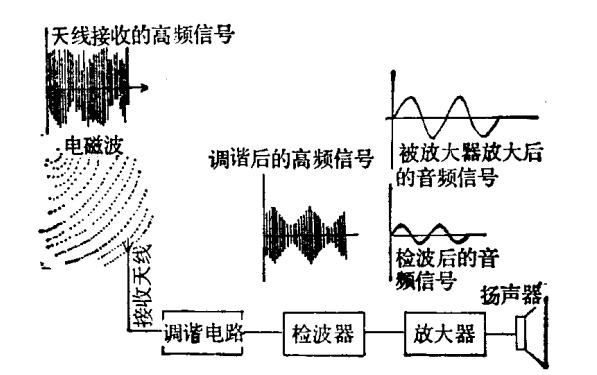
\includegraphics[width=0.8\linewidth]{radio_reception.png}
    \caption{无线电波接收过程示意图}
    \label{fig:radio_reception}
\end{figure}

\subsection{数字广播系统}

数字广播技术的发展展示了无线电技术在信息传播中的应用：

\begin{itemize}[leftmargin=3.5em]
    \item \textbf{数字音频广播}：DAB+技术，VHF频段，CD音质服务
    \item \textbf{数字电视广播}：DTMB标准，UHF频段，高清电视传输
    \item \textbf{卫星广播}：卫星传输，覆盖偏远地区广播服务
    \item \textbf{应急广播}：灾害预警系统，特定频段可靠传输
\end{itemize}

\subsection{导航定位系统}

导航定位系统体现了无线电技术在精确定位中的应用：

\begin{itemize}[leftmargin=3.5em]
    \item \textbf{全球导航}：GPS（美国）、北斗（中国）、GLONASS（俄罗斯）、Galileo（欧洲）
    \item \textbf{区域增强}：WAAS（北美）、EGNOS（欧洲）、MSAS（日本）
    \item \textbf{精密定位}：RTK技术，厘米级定位精度
    \item \textbf{室内定位}：蓝牙、Wi-Fi、UWB技术，室内导航
\end{itemize}

\section{雷达与遥感应用}

无线电技术在雷达与遥感领域的应用：

\subsection{气象雷达}

气象雷达技术展示了无线电技术在气象监测中的应用：

\begin{itemize}[leftmargin=3.5em]
    \item \textbf{S波段雷达}：2.7--2.9GHz，降水监测
    \item \textbf{C波段雷达}：5.3--5.5GHz，天气监测
    \item \textbf{X波段雷达}：9.3--9.5GHz，短距离监测
\end{itemize}

\subsection{航空雷达}

航空雷达技术体现了无线电技术在航空安全中的应用：

\begin{itemize}[leftmargin=3.5em]
    \item \textbf{一次雷达}：L波段，目标探测
    \item \textbf{二次雷达}：1090MHz，应答识别
    \item \textbf{气象雷达}：C波段，机载气象监测
\end{itemize}

\subsection{遥感监测}

遥感监测技术展示了无线电技术在环境监测中的应用：

\begin{itemize}[leftmargin=3.5em]
    \item \textbf{环境监测}：多频段遥感，污染监测
    \item \textbf{资源勘探}：地质雷达，矿产资源探测
    \item \textbf{灾害预警}：遥感监测，灾害评估
\end{itemize}

\section{科学研究应用}

无线电技术在科学研究领域的应用：

\subsection{射电天文}

射电天文研究展示了无线电技术在宇宙探索中的应用：

\begin{itemize}[leftmargin=3.5em]
    \item \textbf{低频射电}：30--300MHz，宇宙背景辐射
    \item \textbf{微波背景}：1--100GHz，宇宙微波背景辐射
    \item \textbf{脉冲星研究}：400MHz--10GHz，脉冲星观测
\end{itemize}

\subsection{空间探测}

空间探测技术体现了无线电技术在深空探索中的应用：

\begin{itemize}[leftmargin=3.5em]
    \item \textbf{深空通信}：2GHz、8GHz，深空探测器通信
    \item \textbf{行星探测}：多频段，行星表面探测
    \item \textbf{空间天气}：太阳射电监测，空间天气预报
\end{itemize}

\subsection{地球物理研究}

地球物理研究展示了无线电技术在地球科学研究中的应用：

\begin{itemize}[leftmargin=3.5em]
    \item \textbf{电离层研究}：1--30MHz，电离层特性研究
    \item \textbf{地磁监测}：VLF频段，地磁场变化监测
    \item \textbf{地震研究}：电磁异常监测，地震前兆研究
\end{itemize}

\chapter{中国技术成就}

本章介绍中国在无线电技术领域的重要成就和贡献，包括导航系统、移动通信、广播技术和前沿技术探索等方面。了解中国技术成就有助于理解我国在无线电领域的发展水平。

中国在无线电技术领域的重要成就和贡献：

\section{导航系统成就}

中国在导航系统领域取得的重大成就：

\begin{itemize}[leftmargin=3.5em]
    \item \textbf{北斗导航系统}：建成全球卫星导航系统，定位精度达到厘米级
    \item \textbf{地基增强}：建成全国范围的高精度定位服务网络
    \item \textbf{应用推广}：在交通、农业、测绘等领域广泛应用
\end{itemize}

\section{移动通信成就}

中国在移动通信技术领域的突出贡献：

\begin{itemize}[leftmargin=3.5em]
    \item \textbf{5G技术}：在5G标准制定中发挥重要作用，建成全球最大5G网络
    \item \textbf{设备制造}：华为、中兴等企业在全球市场占据重要地位
    \item \textbf{网络建设}：实现全国范围的4G/5G网络覆盖
\end{itemize}

\section{广播技术成就}

中国在广播技术领域的重要突破：

\begin{itemize}[leftmargin=3.5em]
    \item \textbf{数字电视}：制定具有自主知识产权的DTMB标准
    \item \textbf{应急广播}：建成全国应急广播体系
    \item \textbf{卫星广播}：建成覆盖全国的卫星广播网络
\end{itemize}

\section{前沿技术探索}

中国在前沿无线电技术领域的积极探索：

\begin{itemize}[leftmargin=3.5em]
    \item \textbf{量子通信}：在量子通信技术领域取得重要突破
    \item \textbf{太赫兹技术}：开展太赫兹通信技术研究
    \item \textbf{空天地一体化}：推进卫星与地面网络融合
\end{itemize}

\chapter{未来发展趋势}

本章展望无线电技术的未来发展趋势，包括技术融合、智能技术应用、绿色通信和空天地一体化等方向。了解未来趋势有助于把握技术发展方向。

无线电技术未来的重要发展趋势：

\section{技术融合趋势}

技术融合是无线电技术发展的重要方向：

\begin{itemize}[leftmargin=3.5em]
    \item \textbf{通信与计算融合}：通信技术与边缘计算、云计算深度融合
    \item \textbf{感知与通信融合}：雷达感知与通信功能一体化设计
    \item \textbf{空天地一体化}：卫星、空中平台与地面网络协同
    \item \textbf{人工智能赋能}：AI技术在无线电各环节深度应用
\end{itemize}

\section{频谱扩展趋势}

频谱资源的扩展是无线电技术发展的关键：

\begin{itemize}[leftmargin=3.5em]
    \item \textbf{毫米波频段}：24-100GHz频段技术成熟和应用
    \item \textbf{太赫兹频段}：0.1-10THz频段技术探索和突破
    \item \textbf{可见光通信}：利用可见光频谱进行高速通信
    \item \textbf{水下通信}：发展水下声波和电磁波通信技术
\end{itemize}

\section{绿色节能趋势}

绿色节能是无线电技术可持续发展的重要保障：

\begin{itemize}[leftmargin=3.5em]
    \item \textbf{能效提升}：单位比特传输能耗持续降低
    \item \textbf{材料创新}：新型低损耗材料应用
    \item \textbf{架构优化}：网络架构和协议优化降低能耗
    \item \textbf{可再生能源}：太阳能等可再生能源在设备中应用
\end{itemize}

\section{新兴技术趋势}

无线电技术的新兴发展方向：

\begin{itemize}[leftmargin=3.5em]
    \item \textbf{智能频谱共享}：认知无线电技术实现动态频谱分配
    \item \textbf{量子通信}：基于量子原理的新型通信技术
\end{itemize}

\chapter{技术挑战与机遇}

本章分析无线电技术发展面临的重要挑战和机遇，包括技术挑战、应用挑战和发展机遇等方面。了解挑战与机遇有助于制定技术发展策略。

无线电技术发展面临的重要挑战和机遇：

\section{技术挑战}

无线电技术发展面临的主要技术挑战：

\begin{itemize}[leftmargin=3.5em]
    \item \textbf{频谱资源紧张}：可用频谱资源日益稀缺
    \item \textbf{干扰管理复杂}：多系统共存干扰问题突出
    \item \textbf{安全威胁增加}：网络安全和隐私保护挑战
    \item \textbf{能耗压力增大}：设备数量和流量增长带来能耗压力
\end{itemize}

\section{发展机遇}

无线电技术发展面临的重要发展机遇：

\begin{itemize}[leftmargin=3.5em]
    \item \textbf{智能技术赋能}：人工智能为无线电技术带来新突破
    \item \textbf{新频段开放}：太赫兹等新频段的开发和利用
    \item \textbf{标准化进展}：全球统一标准促进技术创新
    \item \textbf{应用场景拓展}：5G、物联网等新应用推动技术进步
\end{itemize}

\section{应对策略}

面对挑战和机遇，无线电技术发展的应对策略：

\begin{itemize}[leftmargin=3.5em]
    \item \textbf{技术创新}：持续推动核心技术创新
    \item \textbf{标准制定}：积极参与国际标准制定
    \item \textbf{生态构建}：构建开放合作的产业生态
    \item \textbf{人才培养}：加强专业人才培养和储备
\end{itemize}

\chapter{理论基础与教育}

本章介绍无线电技术的理论体系和教育体系，包括基础理论、教育资源和学习方法。理论基础是技术创新的源泉，教育是人才培养的关键。

\section{无线电技术理论体系}

无线电技术的基础理论体系包括：

\begin{itemize}[leftmargin=3.5em]
    \item \textbf{电磁场理论}：麦克斯韦方程组和电磁波理论
    \item \textbf{电路理论}：线性电路和非线性电路分析
    \item \textbf{信号处理理论}：信号的变换、滤波和处理
    \item \textbf{系统理论}：系统的建模、分析和设计
\end{itemize}

\section{无线电技术的发展历程}

无线电技术的发展经历了从理论建立到技术应用的历程：

\begin{itemize}[leftmargin=3.5em]
    \item \textbf{理论奠基}：19世纪电磁场理论的建立
    \item \textbf{实验验证}：赫兹实验证实电磁波存在
    \item \textbf{技术发展}：调制解调技术的不断完善
    \item \textbf{理论深化}：现代信号处理和系统理论的发展
\end{itemize}

\section{无线电技术的基础理论价值}

无线电技术的基础理论具有重要的科学价值：

\begin{itemize}[leftmargin=3.5em]
    \item \textbf{理论完整性}：建立了完整的电磁场理论体系
    \item \textbf{数学工具}：发展了傅里叶分析、复变函数等数学工具
    \item \textbf{工程应用}：为通信、雷达、导航等技术提供理论基础
    \item \textbf{科学研究}：推动了物理学、数学、工程学等多学科发展
\end{itemize}

无线电技术的基础理论不仅是技术应用的基石，也是科学进步的重要推动力。通过深入理解这些基础理论，可以更好地把握无线电技术的发展方向，推动技术创新和应用拓展。

\section{无线电技术的基础理论特点}

无线电技术的基础理论具有以下特点：

\begin{itemize}[leftmargin=3.5em]
    \item \textbf{理论系统性}：建立了完整的电磁场理论体系
    \item \textbf{数学严谨性}：基于严格的数学推导和证明
    \item \textbf{工程实用性}：理论可以直接指导工程实践
    \item \textbf{发展持续性}：理论体系不断发展和完善
\end{itemize}

这些特点使得无线电技术的基础理论具有持久的科学价值和广泛的应用前景。

\section{基础理论的应用示例}

无线电技术的基础理论在以下领域具有重要应用价值：

\textbf{频谱资源管理}：
\begin{itemize}[leftmargin=3.5em]
    \item \textbf{频段划分原理}：基于电磁波传播特性的频段科学划分
    \item \textbf{频谱效率理论}：香农定理指导下的频谱利用优化
    \item \textbf{干扰分析基础}：电磁兼容性理论的应用
\end{itemize}

\textbf{通信系统设计}：
\begin{itemize}[leftmargin=3.5em]
    \item \textbf{调制解调原理}：信息论在通信系统中的应用
    \item \textbf{信道编码理论}：纠错编码和信道容量的理论基础
    \item \textbf{多址接入技术}：资源分配和调度算法的理论支撑
\end{itemize}

\section{实验与教育}

无线电技术的基础实验和教育资源：

\textbf{基础实验项目}：
\begin{itemize}[leftmargin=3.5em]
    \item \textbf{天线制作实验}：使用铜线制作偶极子天线，测试接收效果
    \item \textbf{信号检测实验}：使用示波器观察AM/FM广播信号波形
    \item \textbf{频率测量实验}：使用频率计测量本地广播电台频率
    \item \textbf{场强测量实验}：使用场强仪测量不同位置的信号强度
\end{itemize}

\textbf{教学资源平台}：
\begin{itemize}[leftmargin=3.5em]
    \item \textbf{在线课程}：各大高校的无线电技术在线课程
    \item \textbf{实验平台}：虚拟实验平台和远程实验系统
    \item \textbf{教材资源}：专业教材和参考书籍
    \item \textbf{开源项目}：开源硬件和软件项目
\end{itemize}

\textbf{理论学习方法}：
\begin{itemize}[leftmargin=3.5em]
    \item \textbf{理论联系实际}：将基础理论与实际应用相结合
    \item \textbf{数学工具运用}：熟练掌握相关数学工具和方法
    \item \textbf{系统思维培养}：建立完整的无线电技术知识体系
    \item \textbf{创新能力培养}：基于理论基础的创新思维训练
\end{itemize}

\textbf{科普教育推广}：
\begin{itemize}[leftmargin=3.5em]
    \item \textbf{青少年科普}：无线电知识普及，科技竞赛
    \item \textbf{公众教育}：科普讲座、科技馆展览
    \item \textbf{业余无线电}：业余无线电爱好者活动
    \item \textbf{技术培训}：职业技能培训和认证
\end{itemize}


\backmatter

\chapter{参考书籍}

\begin{enumerate}[leftmargin=3.5em]
    \item 白之卿, 沈承衡. \textit{从矿石机到二管机}. 人民邮电出版社, 15045.总883-无214
    \item 朱蔼初. \textit{看图学装收音机}. 少年儿童出版社, 1984年, 上海
    \item 冯报本. \textit{矿石收音机}. 人民邮电出版社, 15045.总319-无61
    \item 汪午生, 金海初, 柴铿. \textit{矿石收音机}. 
    \item 王汉祯. \textit{少年无线电入门}. 福建科学技术出版社, 1983年, 15211.29
    \item 陈鹏飞. \textit{无电源收音机}. 黑龙江科学技术出版社, 1985年, 15217.170
    \item 陈鹏飞. \textit{晶体管二、三管收音机}. 黑龙江科学技术出版社, 1985年, 15217.174
    \item 吴志功, 王昌辉, 耿文学, 洪水平, 廖秉权. \textit{青年无线电实用手册}. 中国青年出版社
    \item 俞锡良. \textit{业余电子管收音机设计}. 人民邮电出版社, 15045.总1379-无381
\end{enumerate}

\chapter{术语表}

\begin{description}
    \item[电磁波] 由变化的电场和磁场相互激发而形成的波动现象，以光速在空间传播
    \item[无线电波] 电磁波频谱中频率较低的部分，频率范围从3kHz到300GHz
    \item[调制] 将信息信号加载到载波上的过程，是无线电通信的核心技术
    \item[解调] 从已调制信号中恢复原始信息信号的过程
    \item[天线] 用于发射和接收电磁波的设备，实现电磁波与电信号之间的转换
    \item[频谱] 信号在频域的分布特性，用于信号的分析和处理
    \item[带宽] 信号或系统能够有效工作的频率范围
    \item[增益] 天线在特定方向上的辐射或接收能力，相对于参考天线的增益
    \item[方向性] 天线在不同方向上的辐射或接收能力不同的特性
    \item[阻抗] 天线的输入阻抗，需要与传输线和接收电路的阻抗匹配
    \item[驻波比] 衡量天线阻抗匹配程度的指标，驻波比越接近1，匹配越好
    \item[传播模式] 无线电波在空间中的传播方式，包括地波、天波、空间波等
    \item[衰落] 无线电信号在传输过程中因多径效应等因素导致的信号强度起伏
    \item[多径效应] 信号通过多条路径到达接收端，导致信号干涉的现象
    \item[多普勒效应] 由于发射源和接收端之间的相对运动，导致信号频率发生变化的现象
    \item[MIMO] 多输入多输出技术，通过多个天线同时收发信号，提高系统容量和可靠性
    \item[OFDM] 正交频分复用技术，将宽带信号分解为多个窄带子载波并行传输
    \item[SDR] 软件定义无线电，通过软件配置实现不同通信标准的无线电系统
    \item[认知无线电] 能够感知周围频谱环境，动态调整工作参数的智能无线电技术
    \item[太赫兹通信] 使用0.1-10THz频段的通信技术，支持超高容量传输
\end{description}

\printindex

\end{document}